\documentclass[10pt,a4paper,oneside]{article}

\usepackage[margin=2.5cm,top=3cm]{geometry}
\usepackage{amsmath, amssymb}
\numberwithin{equation}{section} %Numbering of our equations per section
\usepackage{algorithm, algpseudocode}
\usepackage{fancyhdr}
\usepackage{graphicx}
\usepackage{lastpage}
\usepackage{setspace}
\usepackage[hyphens]{url}
\usepackage{mdframed}
\usepackage{xcolor}
\definecolor{commentgreen}{RGB}{2,112,10}
\usepackage{tabularx}
\usepackage{appendix}
\usepackage{courier} %% Sets font for listing as Courier.
\usepackage{verbatim}
\usepackage{alltt}

\usepackage{listings}
\lstset{
  frame=none,
  xleftmargin=2pt,
  stepnumber=1,
  numbers=left,
  numbersep=5pt,
  numberstyle=\ttfamily\tiny\color[gray]{0.3},
  belowcaptionskip=\bigskipamount,
  captionpos=b,
  escapeinside={*'}{'*},
  language=haskell,
  tabsize=2,
  emphstyle={\bf},
  commentstyle=\it\color{commentgreen},
  stringstyle=\mdseries\rmfamily\color{red},
  showspaces=false,
  keywordstyle=\bfseries\rmfamily\color{blue},
  columns=flexible,
  basicstyle=\small\ttfamily,
  showstringspaces=false,
  morecomment=[l]\%,
  frame = trBL,
  firstnumber = 1
}

\usepackage[hidelinks]{hyperref}

\newcommand{\blue}[1]{\textcolor{blue}{#1}}
\newcommand{\green}[1]{\textcolor{green}{#1}}
\newcommand{\red}[1]{\textcolor{red}{#1}}
\newcommand{\bordertext}[1]{%
\smallskip\par%
\noindent\fbox{%
    \parbox{\dimexpr\linewidth-2\fboxsep-2\fboxrule}{#1}%
}\smallskip%
}
\setlength{\parindent}{0cm}

\fancyhf{}
\pagestyle{fancy}
\renewcommand{\headrulewidth}{0.2pt}
\pagenumbering{roman}
\fancyfoot[c]{\thepage}

\begin{document}

\thispagestyle{empty}

\begin{spacing}{2}
	\begin{center}
		
\includegraphics[scale = 0.45]{latex/assets/haskell-logo.png}
	\end{center}
	\vspace{5mm}
	\begin{center}
		\textbf{\begin{LARGE}
		Haskell Tutorial
		\end{LARGE}}
		\vspace{4mm}
	\end{center}
	\begin{center}
		{\large A guide to Haskell basics}\\
		\vspace{20mm}
	\end{center}
	\begin{center}
		\textbf{{\large Ruben Saunders}}
		\vspace{20mm}
	\end{center}
\end{spacing}

\pagenumbering{roman}


\tableofcontents
\newpage

\pagenumbering{arabic}
\fancyfoot[c]{Page \thepage \hspace{1pt} of \pageref{LastPage}}

\section{Introduction}
\label{sec:introduction}
Haskell is a purely functional programming language. The following sections will give a brief overview of Haskell, and how to install it.

\subsection{Language Overview}
In Haskell, everything is a \textit{pure} function - that is, they abide by the Mathematical definition of a function; they map inputs to a unique output.

Data is immutable, meaning that our data types cannot be changed in-place. Combined, this means that there a re few or no side-effects from functions, which make programming more simple.

Haskell is declarative, meaning that the program defines what the issue is, rather than simply giving an algorithm to solve a problem.

Functional programs are easier to verify as we can use maths to verify an algorithm.

\subsection{Installation}
Link: \url{https://www.haskell.org/ghcup/}

I used GHCup to install several components of the Haskell toolchain.

\subsubsection{The Haskell Toolchain}
The Haskell Toolchain consists of several useful tools for Haskell compilatio and development:

\begin{itemize}
  \item \textbf{GHC} - the Glasgow Haskell Compiler;
  \item \textbf{cabal-install} - Cabal installation tool for managing Haskell software;
  \item \textbf{Stack} - a cross-platform proram for developing Haskell projects;
  \begin{itemize}
    \item \textbf{Msys2} - provides a UNIX shell and environment which is necessary for executing configuration scripts.
  \end{itemize}
  \item \textbf{haskell-language-server} - a language server which may be integrated into an IDE;
\end{itemize}

\subsubsection{Install Command}
The command to use on Windows (in a normal Powershell instance) is

% Credit: https://github.com/rmainer/latex-listings-powershell/
\definecolor{lst-gray}{rgb}{0.98,0.98,0.98}
\definecolor{lst-blue}{RGB}{40,0.0,255}
\definecolor{lst-green}{RGB}{65,128,95}
\definecolor{lst-red}{RGB}{200,0,85}

\lstdefinelanguage{PowerShell}{
	morekeywords={
		Add-Content,Add-PSSnapin,Clear-Content,Clear-History,Clear-Host,Clear-Item,Clear-ItemProperty,Clear-Variable,Compare-Object,Connect-PSSession,ConvertFrom-String,Convert-Path,Copy-Item,Copy-ItemProperty,Disable-PSBreakpoint,Disconnect-PSSession,Enable-PSBreakpoint,Enter-PSSession,Exit-PSSession,Export-Alias,Export-Csv,Export-PSSession,ForEach-Object,Format-Custom,Format-Hex,Format-List,Format-Table,Format-Wide,Get-Alias,Get-ChildItem,Get-Clipboard,Get-Command,Get-ComputerInfo,Get-Content,Get-History,Get-Item,Get-ItemProperty,Get-ItemPropertyValue,Get-Job,Get-Location,Get-Member,Get-Module,Get-Process,Get-PSBreakpoint,Get-PSCallStack,Get-PSDrive,Get-PSSession,Get-PSSnapin,Get-Service,Get-TimeZone,Get-Unique,Get-Variable,Get-WmiObject,Group-Object,help,Import-Alias,Import-Csv,Import-Module,Import-PSSession,Invoke-Command,Invoke-Expression,Invoke-History,Invoke-Item,Invoke-RestMethod,Invoke-WebRequest,Invoke-WmiMethod,Measure-Object,mkdir,Move-Item,Move-ItemProperty,New-Alias,New-Item,New-Module,New-PSDrive,New-PSSession,New-PSSessionConfigurationFile,New-Variable,Out-GridView,Out-Host,Out-Printer,Pop-Location,powershell_ise.exe,Push-Location,Receive-Job,Receive-PSSession,Remove-Item,Remove-ItemProperty,Remove-Job,Remove-Module,Remove-PSBreakpoint,Remove-PSDrive,Remove-PSSession,Remove-PSSnapin,Remove-Variable,Remove-WmiObject,Rename-Item,Rename-ItemProperty,Resolve-Path,Resume-Job,Select-Object,Select-String,Set-Alias,Set-Clipboard,Set-Content,Set-Item,Set-ItemProperty,Set-Location,Set-PSBreakpoint,Set-TimeZone,Set-Variable,Set-WmiInstance,Show-Command,Sort-Object,Start-Job,Start-Process,Start-Service,Start-Sleep,Stop-Job,Stop-Process,Stop-Service,Suspend-Job,Tee-Object,Trace-Command,Wait-Job,Where-Object,Write-Output
	},
	morekeywords={
		Add-AppxPackage,Add-AppxProvisionedPackage,Add-AppxVolume,Add-BitsFile,Add-CertificateEnrollmentPolicyServer,Add-Computer,Add-Content,Add-History,Add-JobTrigger,Add-KdsRootKey,Add-LocalGroupMember,Add-Member,Add-PSSnapin,Add-Type,Add-WindowsCapability,Add-WindowsDriver,Add-WindowsImage,Add-WindowsPackage,Checkpoint-Computer,Clear-Content,Clear-EventLog,Clear-History,Clear-Item,Clear-ItemProperty,Clear-KdsCache,Clear-RecycleBin,Clear-Tpm,Clear-Variable,Clear-WindowsCorruptMountPoint,Compare-Object,Complete-BitsTransfer,Complete-DtiagnosticTransaction,Complete-Transaction,Confirm-SecureBootUEFI,Connect-PSSession,Connect-WSMan,ConvertFrom-Csv,ConvertFrom-Json,ConvertFrom-SecureString,ConvertFrom-String,ConvertFrom-StringData,Convert-Path,Convert-String,ConvertTo-Csv,ConvertTo-Html,ConvertTo-Json,ConvertTo-ProcessMitigationPolicy,ConvertTo-SecureString,ConvertTo-TpmOwnerAuth,ConvertTo-Xml,Copy-Item,Copy-ItemProperty,Debug-Job,Debug-Process,Debug-Runspace,Disable-AppBackgroundTaskDiagnosticLog,Disable-ComputerRestore,Disable-JobTrigger,Disable-LocalUser,Disable-PSBreakpoint,Disable-PSRemoting,Disable-PSSessionConfiguration,Disable-RunspaceDebug,Disable-ScheduledJob,Disable-TlsCipherSuite,Disable-TlsEccCurve,Disable-TlsSessionTicketKey,Disable-TpmAutoProvisioning,Disable-WindowsErrorReporting,Disable-WindowsOptionalFeature,Disable-WSManCredSSP,Disconnect-PSSession,Disconnect-WSMan,Dismount-AppxVolume,Dismount-WindowsImage,Enable-AppBackgroundTaskDiagnosticLog,Enable-ComputerRestore,Enable-JobTrigger,Enable-LocalUser,Enable-PSBreakpoint,Enable-PSRemoting,Enable-PSSessionConfiguration,Enable-RunspaceDebug,Enable-ScheduledJob,Enable-TlsCipherSuite,Enable-TlsEccCurve,Enable-TlsSessionTicketKey,Enable-TpmAutoProvisioning,Enable-WindowsErrorReporting,Enable-WindowsOptionalFeature,Enable-WSManCredSSP,Enter-PSHostProcess,Enter-PSSession,Exit-PSHostProcess,Exit-PSSession,Expand-WindowsCustomDataImage,Expand-WindowsImage,Export-Alias,Export-BinaryMiLog,Export-Certificate,Export-Clixml,Export-Console,Export-Counter,Export-Csv,Export-FormatData,Export-ModuleMember,Export-PfxCertificate,Export-ProvisioningPackage,Export-PSSession,Export-StartLayout,Export-StartLayoutEdgeAssets,Export-TlsSessionTicketKey,Export-Trace,Export-WindowsCapabilitySource,Export-WindowsDriver,Export-WindowsImage,Find-Package,Find-PackageProvider,ForEach-Object,Format-Custom,Format-List,Format-SecureBootUEFI,Format-Table,Format-Wide,Get-Acl,Get-Alias,Get-AppxDefaultVolume,Get-AppxPackage,Get-AppxPackageManifest,Get-AppxProvisionedPackage,Get-AppxVolume,Get-AuthenticodeSignature,Get-BitsTransfer,Get-Certificate,Get-CertificateAutoEnrollmentPolicy,Get-CertificateEnrollmentPolicyServer,Get-CertificateNotificationTask,Get-ChildItem,Get-CimAssociatedInstance,Get-CimClass,Get-CimInstance,Get-CimSession,Get-Clipboard,Get-CmsMessage,Get-Command,Get-ComputerInfo,Get-ComputerRestorePoint,Get-Content,Get-ControlPanelItem,Get-Counter,Get-Credential,Get-Culture,Get-DAPolicyChange,Get-Date,Get-DeliveryOptimizationLog,Get-DeliveryOptimizationPerfSnap,Get-DeliveryOptimizationPerfSnapThisMonth,Get-DeliveryOptimizationStatus,Get-DODownloadMode,Get-DOPercentageMaxBackgroundBandwidth,Get-DOPercentageMaxForegroundBandwidth,Get-Event,Get-EventLog,Get-EventSubscriber,Get-ExecutionPolicy,Get-FormatData,Get-Help,Get-History,Get-Host,Get-HotFix,Get-Item,Get-ItemProperty,Get-ItemPropertyValue,Get-Job,Get-JobTrigger,Get-KdsConfiguration,Get-KdsRootKey,Get-LocalGroup,Get-LocalGroupMember,Get-LocalUser,Get-Location,Get-Member,Get-Module,Get-Package,Get-PackageProvider,Get-PackageSource,Get-PfxCertificate,Get-PfxData,Get-PmemDisk,Get-PmemPhysicalDevice,Get-PmemUnusedRegion,Get-Process,Get-ProcessMitigation,Get-ProvisioningPackage,Get-PSBreakpoint,Get-PSCallStack,Get-PSDrive,Get-PSHostProcessInfo,Get-PSProvider,Get-PSReadlineKeyHandler,Get-PSReadlineOption,Get-PSSession,Get-PSSessionCapability,Get-PSSessionConfiguration,Get-PSSnapin,Get-Random,Get-Runspace,Get-RunspaceDebug,Get-ScheduledJob,Get-ScheduledJobOption,Get-SecureBootPolicy,Get-SecureBootUEFI,Get-Service,Get-TimeZone,Get-TlsCipherSuite,Get-TlsEccCurve,Get-Tpm,Get-TpmEndorsementKeyInfo,Get-TpmSupportedFeature,Get-TraceSource,Get-Transaction,Get-TroubleshootingPack,Get-TrustedProvisioningCertificate,Get-TypeData,Get-UICulture,Get-Unique,Get-Variable,Get-WIMBootEntry,Get-WinAcceptLanguageFromLanguageListOptOut,Get-WinCultureFromLanguageListOptOut,Get-WinDefaultInputMethodOverride,Get-WindowsCapability,Get-WindowsDeveloperLicense,Get-WindowsDriver,Get-WindowsEdition,Get-WindowsErrorReporting,Get-WindowsImage,Get-WindowsImageContent,Get-WindowsOptionalFeature,Get-WindowsPackage,Get-WindowsSearchSetting,Get-WinEvent,Get-WinHomeLocation,Get-WinLanguageBarOption,Get-WinSystemLocale,Get-WinUILanguageOverride,Get-WinUserLanguageList,Get-WmiObject,Get-WSManCredSSP,Get-WSManInstance,Group-Object,Import-Alias,Import-BinaryMiLog,Import-Certificate,Import-Clixml,Import-Counter,Import-Csv,Import-LocalizedData,Import-Module,Import-PackageProvider,Import-PfxCertificate,Import-PSSession,Import-StartLayout,Import-TpmOwnerAuth,Initialize-PmemPhysicalDevice,Initialize-Tpm,Install-Package,Install-PackageProvider,Install-ProvisioningPackage,Install-TrustedProvisioningCertificate,Invoke-CimMethod,Invoke-Command,Invoke-CommandInDesktopPackage,Invoke-DscResource,Invoke-Expression,Invoke-History,Invoke-Item,Invoke-RestMethod,Invoke-TroubleshootingPack,Invoke-WebRequest,Invoke-WmiMethod,Invoke-WSManAction,Join-DtiagnosticResourceManager,Join-Path,Limit-EventLog,Measure-Command,Measure-Object,Mount-AppxVolume,Mount-WindowsImage,Move-AppxPackage,Move-Item,Move-ItemProperty,New-Alias,New-CertificateNotificationTask,New-CimInstance,New-CimSession,New-CimSessionOption,New-DtiagnosticTransaction,New-Event,New-EventLog,New-FileCatalog,New-Item,New-ItemProperty,New-JobTrigger,New-LocalGroup,New-LocalUser,New-Module,New-ModuleManifest,New-NetIPsecAuthProposal,New-NetIPsecMainModeCryptoProposal,New-NetIPsecQuickModeCryptoProposal,New-Object,New-PmemDisk,New-ProvisioningRepro,New-PSDrive,New-PSRoleCapabilityFile,New-PSSession,New-PSSessionConfigurationFile,New-PSSessionOption,New-PSTransportOption,New-PSWorkflowExecutionOption,New-ScheduledJobOption,New-SelfSignedCertificate,New-Service,New-TimeSpan,New-TlsSessionTicketKey,New-Variable,New-WebServiceProxy,New-WindowsCustomImage,New-WindowsImage,New-WinEvent,New-WinUserLanguageList,New-WSManInstance,New-WSManSessionOption,Optimize-AppxProvisionedPackages,Optimize-WindowsImage,Out-Default,Out-File,Out-GridView,Out-Host,Out-Null,Out-Printer,Out-String,Pop-Location,Protect-CmsMessage,Publish-DscConfiguration,Push-Location,Read-Host,Receive-DtiagnosticTransaction,Receive-Job,Receive-PSSession,Register-ArgumentCompleter,Register-CimIndicationEvent,Register-EngineEvent,Register-ObjectEvent,Register-PackageSource,Register-PSSessionConfiguration,Register-ScheduledJob,Register-WmiEvent,Remove-AppxPackage,Remove-AppxProvisionedPackage,Remove-AppxVolume,Remove-BitsTransfer,Remove-CertificateEnrollmentPolicyServer,Remove-CertificateNotificationTask,Remove-CimInstance,Remove-CimSession,Remove-Computer,Remove-Event,Remove-EventLog,Remove-Item,Remove-ItemProperty,Remove-Job,Remove-JobTrigger,Remove-LocalGroup,Remove-LocalGroupMember,Remove-LocalUser,Remove-Module,Remove-PmemDisk,Remove-PSBreakpoint,Remove-PSDrive,Remove-PSReadlineKeyHandler,Remove-PSSession,Remove-PSSnapin,Remove-TypeData,Remove-Variable,Remove-WindowsCapability,Remove-WindowsDriver,Remove-WindowsImage,Remove-WindowsPackage,Remove-WmiObject,Remove-WSManInstance,Rename-Computer,Rename-Item,Rename-ItemProperty,Rename-LocalGroup,Rename-LocalUser,Repair-WindowsImage,Reset-ComputerMachinePassword,Resolve-DnsName,Resolve-Path,Restart-Computer,Restart-Service,Restore-Computer,Resume-BitsTransfer,Resume-Job,Resume-ProvisioningSession,Resume-Service,Save-Help,Save-Package,Save-WindowsImage,Select-Object,Select-String,Select-Xml,Send-DtiagnosticTransaction,Send-MailMessage,Set-Acl,Set-Alias,Set-AppBackgroundTaskResourcePolicy,Set-AppxDefaultVolume,Set-AppXProvisionedDataFile,Set-AuthenticodeSignature,Set-BitsTransfer,Set-CertificateAutoEnrollmentPolicy,Set-CimInstance,Set-Clipboard,Set-Content,Set-Culture,Set-Date,Set-DODownloadMode,Set-DOPercentageMaxBackgroundBandwidth,Set-DOPercentageMaxForegroundBandwidth,Set-DscLocalConfigurationManager,Set-ExecutionPolicy,Set-Item,Set-ItemProperty,Set-JobTrigger,Set-KdsConfiguration,Set-LocalGroup,Set-LocalUser,Set-Location,Set-PackageSource,Set-ProcessMitigation,Set-PSBreakpoint,Set-PSDebug,Set-PSReadlineKeyHandler,Set-PSReadlineOption,Set-PSSessionConfiguration,Set-ScheduledJob,Set-ScheduledJobOption,Set-SecureBootUEFI,Set-Service,Set-StrictMode,Set-TimeZone,Set-TpmOwnerAuth,Set-TraceSource,Set-Variable,Set-WinAcceptLanguageFromLanguageListOptOut,Set-WinCultureFromLanguageListOptOut,Set-WinDefaultInputMethodOverride,Set-WindowsEdition,Set-WindowsProductKey,Set-WindowsSearchSetting,Set-WinHomeLocation,Set-WinLanguageBarOption,Set-WinSystemLocale,Set-WinUILanguageOverride,Set-WinUserLanguageList,Set-WmiInstance,Set-WSManInstance,Set-WSManQuickConfig,Show-Command,Show-ControlPanelItem,Show-EventLog,Show-WindowsDeveloperLicenseRegistration,Sort-Object,Split-Path,Split-WindowsImage,Start-BitsTransfer,Start-DscConfiguration,Start-DtiagnosticResourceManager,Start-Job,Start-Process,Start-Service,Start-Sleep,Start-Transaction,Start-Transcript,Stop-Computer,Stop-DtiagnosticResourceManager,Stop-Job,Stop-Process,Stop-Service,Stop-Transcript,Suspend-BitsTransfer,Suspend-Job,Suspend-Service,Switch-Certificate,Tee-Object,Test-Certificate,Test-ComputerSecureChannel,Test-Connection,Test-DscConfiguration,Test-FileCatalog,Test-KdsRootKey,Test-ModuleManifest,Test-Path,Test-PSSessionConfigurationFile,Test-WSMan,Trace-Command,Unblock-File,Unblock-Tpm,Undo-DtiagnosticTransaction,Undo-Transaction,Uninstall-Package,Uninstall-ProvisioningPackage,Uninstall-TrustedProvisioningCertificate,Unprotect-CmsMessage,Unregister-Event,Unregister-PackageSource,Unregister-PSSessionConfiguration,Unregister-ScheduledJob,Unregister-WindowsDeveloperLicense,Update-FormatData,Update-Help,Update-List,Update-TypeData,Update-WIMBootEntry,Use-Transaction,Use-WindowsUnattend,Wait-Debugger,Wait-Event,Wait-Job,Wait-Process,Where-Object,Write-Debug,Write-Error,Write-EventLog,Write-Host,Write-Information,Write-Output,Write-Progress,Write-Verbose,Write-Warning
	},
	morekeywords={
		Add-BitLockerKeyProtector,Add-DnsClientNrptRule,Add-DtcClusterTMMapping,Add-EtwTraceProvider,Add-InitiatorIdToMaskingSet,Add-MpPreference,Add-NetEventNetworkAdapter,Add-NetEventPacketCaptureProvider,Add-NetEventProvider,Add-NetEventVFPProvider,Add-NetEventVmNetworkAdapter,Add-NetEventVmSwitch,Add-NetEventVmSwitchProvider,Add-NetEventWFPCaptureProvider,Add-NetIPHttpsCertBinding,Add-NetLbfoTeamMember,Add-NetLbfoTeamNic,Add-NetNatExternalAddress,Add-NetNatStaticMapping,Add-NetSwitchTeamMember,Add-Odbsn,Add-PartitionAccessPath,Add-PhysicalDisk,Add-Printer,Add-PrinterDriver,Add-PrinterPort,Add-StorageFaultDomain,Add-TargetPortToMaskingSet,Add-VirtualDiskToMaskingSet,Add-VpnConnection,Add-VpnConnectionRoute,Add-VpnConnectionTriggerApplication,Add-VpnConnectionTriggerDnsConfiguration,Add-VpnConnectionTriggerTrustedNetwork,AfterAll,AfterEach,Assert-MockCalled,Assert-VerifiableMocks,Backup-BitLockerKeyProtector,BackupToAAD-BitLockerKeyProtector,BeforeAll,BeforeEach,Block-FileShareAccess,Block-SmbShareAccess,Clear-BitLockerAutoUnlock,Clear-Disk,Clear-DnsClientCache,Clear-FileStorageTier,Clear-Host,Clear-PcsvDeviceLog,Clear-StorageDiagnosticInfo,Close-SmbOpenFile,Close-SmbSession,Compress-Archive,Configuration,Connect-IscsiTarget,Connect-VirtualDisk,Context,convert,ConvertFrom-SddlString,Copy-NetFirewallRule,Copy-NetIPsecMainModeCryptoSet,Copy-NetIPsecMainModeRule,Copy-NetIPsecPhase1AuthSet,Copy-NetIPsecPhase2AuthSet,Copy-NetIPsecQuickModeCryptoSet,Copy-NetIPsecRule,Debug-FileShare,Debug-MMAppPrelaunch,Debug-StorageSubSystem,Debug-Volume,Describe,Disable-BitLocker,Disable-BitLockerAutoUnlock,Disable-DAManualEntryPointSelection,Disable-Dsebug,Disable-MMAgent,Disable-NetAdapter,Disable-NetAdapterBinding,Disable-NetAdapterChecksumOffload,Disable-NetAdapterEncapsulatedPacketTaskOffload,Disable-NetAdapterIPsecOffload,Disable-NetAdapterLso,Disable-NetAdapterPacketDirect,Disable-NetAdapterPowerManagement,Disable-NetAdapterQos,Disable-NetAdapterRdma,Disable-NetAdapterRsc,Disable-NetAdapterRss,Disable-NetAdapterSriov,Disable-NetAdapterVmq,Disable-NetDnsTransitionConfiguration,Disable-NetFirewallRule,Disable-NetIPHttpsProfile,Disable-NetIPsecMainModeRule,Disable-NetIPsecRule,Disable-NetNatTransitionConfiguration,Disable-NetworkSwitchEthernetPort,Disable-NetworkSwitchFeature,Disable-NetworkSwitchVlan,Disable-OdbcPerfCounter,Disable-PhysicalDiskIdentification,Disable-PnpDevice,Disable-PSTrace,Disable-PSWSManCombinedTrace,Disable-ScheduledTask,Disable-SmbDelegation,Disable-StorageEnclosureIdentification,Disable-StorageEnclosurePower,Disable-StorageHighAvailability,Disable-StorageMaintenanceMode,Disable-WdacBidTrace,Disable-WSManTrace,Disconnect-IscsiTarget,Disconnect-VirtualDisk,Dismount-DiskImage,Enable-BitLocker,Enable-BitLockerAutoUnlock,Enable-DAManualEntryPointSelection,Enable-Dsebug,Enable-MMAgent,Enable-NetAdapter,Enable-NetAdapterBinding,Enable-NetAdapterChecksumOffload,Enable-NetAdapterEncapsulatedPacketTaskOffload,Enable-NetAdapterIPsecOffload,Enable-NetAdapterLso,Enable-NetAdapterPacketDirect,Enable-NetAdapterPowerManagement,Enable-NetAdapterQos,Enable-NetAdapterRdma,Enable-NetAdapterRsc,Enable-NetAdapterRss,Enable-NetAdapterSriov,Enable-NetAdapterVmq,Enable-NetDnsTransitionConfiguration,Enable-NetFirewallRule,Enable-NetIPHttpsProfile,Enable-NetIPsecMainModeRule,Enable-NetIPsecRule,Enable-NetNatTransitionConfiguration,Enable-NetworkSwitchEthernetPort,Enable-NetworkSwitchFeature,Enable-NetworkSwitchVlan,Enable-OdbcPerfCounter,Enable-PhysicalDiskIdentification,Enable-PnpDevice,Enable-PSTrace,Enable-PSWSManCombinedTrace,Enable-ScheduledTask,Enable-SmbDelegation,Enable-StorageEnclosureIdentification,Enable-StorageEnclosurePower,Enable-StorageHighAvailability,Enable-StorageMaintenanceMode,Enable-WdacBidTrace,Enable-WSManTrace,Expand-Archive,Export-ODataEndpointProxy,Export-ScheduledTask,Find-Command,Find-DscResource,Find-Module,Find-NetIPsecRule,Find-NetRoute,Find-RoleCapability,Find-Script,Flush-EtwTraceSession,Format-Hex,Format-Volume,Get-AppBackgroundTask,Get-AppxLastError,Get-AppxLog,Get-AutologgerConfig,Get-BitLockerVolume,Get-ClusteredScheduledTask,Get-DAClientExperienceConfiguration,Get-DAConnectionStatus,Get-DAEntryPointTableItem,Get-DedupProperties,Get-Disk,Get-DiskImage,Get-DiskStorageNodeView,Get-DnsClient,Get-DnsClientCache,Get-DnsClientGlobalSetting,Get-DnsClientNrptGlobal,Get-DnsClientNrptPolicy,Get-DnsClientNrptRule,Get-DnsClientServerAddress,Get-DscConfiguration,Get-DscConfigurationStatus,Get-DscLocalConfigurationManager,Get-DscResource,Get-Dtc,Get-DtcAdvancedHostSetting,Get-DtcAdvancedSetting,Get-DtcClusterDefault,Get-DtcClusterTMMapping,Get-Dtefault,Get-DtcLog,Get-DtcNetworkSetting,Get-DtcTransaction,Get-DtcTransactionsStatistics,Get-DtcTransactionsTraceSession,Get-DtcTransactionsTraceSetting,Get-EtwTraceProvider,Get-EtwTraceSession,Get-FileHash,Get-FileIntegrity,Get-FileShare,Get-FileShareAccessControlEntry,Get-FileStorageTier,Get-InitiatorId,Get-InitiatorPort,Get-InstalledModule,Get-InstalledScript,Get-IscsiConnection,Get-IscsiSession,Get-IscsiTarget,Get-IscsiTargetPortal,Get-IseSnippet,Get-LogProperties,Get-MaskingSet,Get-MMAgent,Get-MockDynamicParameters,Get-MpComputerStatus,Get-MpPreference,Get-MpThreat,Get-MpThreatCatalog,Get-MpThreatDetection,Get-NCSIPolicyConfiguration,Get-Net6to4Configuration,Get-NetAdapter,Get-NetAdapterAdvancedProperty,Get-NetAdapterBinding,Get-NetAdapterChecksumOffload,Get-NetAdapterEncapsulatedPacketTaskOffload,Get-NetAdapterHardwareInfo,Get-NetAdapterIPsecOffload,Get-NetAdapterLso,Get-NetAdapterPacketDirect,Get-NetAdapterPowerManagement,Get-NetAdapterQos,Get-NetAdapterRdma,Get-NetAdapterRsc,Get-NetAdapterRss,Get-NetAdapterSriov,Get-NetAdapterSriovVf,Get-NetAdapterStatistics,Get-NetAdapterVmq,Get-NetAdapterVMQQueue,Get-NetAdapterVPort,Get-NetCompartment,Get-NetConnectionProfile,Get-NetDnsTransitionConfiguration,Get-NetDnsTransitionMonitoring,Get-NetEventNetworkAdapter,Get-NetEventPacketCaptureProvider,Get-NetEventProvider,Get-NetEventSession,Get-NetEventVFPProvider,Get-NetEventVmNetworkAdapter,Get-NetEventVmSwitch,Get-NetEventVmSwitchProvider,Get-NetEventWFPCaptureProvider,Get-NetFirewallAddressFilter,Get-NetFirewallApplicationFilter,Get-NetFirewallInterfaceFilter,Get-NetFirewallInterfaceTypeFilter,Get-NetFirewallPortFilter,Get-NetFirewallProfile,Get-NetFirewallRule,Get-NetFirewallSecurityFilter,Get-NetFirewallServiceFilter,Get-NetFirewallSetting,Get-NetIPAddress,Get-NetIPConfiguration,Get-NetIPHttpsConfiguration,Get-NetIPHttpsState,Get-NetIPInterface,Get-NetIPseospSetting,Get-NetIPsecMainModeCryptoSet,Get-NetIPsecMainModeRule,Get-NetIPsecMainModeSA,Get-NetIPsecPhase1AuthSet,Get-NetIPsecPhase2AuthSet,Get-NetIPsecQuickModeCryptoSet,Get-NetIPsecQuickModeSA,Get-NetIPsecRule,Get-NetIPv4Protocol,Get-NetIPv6Protocol,Get-NetIsatapConfiguration,Get-NetLbfoTeam,Get-NetLbfoTeamMember,Get-NetLbfoTeamNic,Get-NetNat,Get-NetNatExternalAddress,Get-NetNatGlobal,Get-NetNatSession,Get-NetNatStaticMapping,Get-NetNatTransitionConfiguration,Get-NetNatTransitionMonitoring,Get-NetNeighbor,Get-NetOffloadGlobalSetting,Get-NetPrefixPolicy,Get-NetQosPolicy,Get-NetRoute,Get-NetSwitchTeam,Get-NetSwitchTeamMember,Get-NetTCPConnection,Get-NetTCPSetting,Get-NetTeredoConfiguration,Get-NetTeredoState,Get-NetTransportFilter,Get-NetUDPEndpoint,Get-NetUDPSetting,Get-NetworkSwitchEthernetPort,Get-NetworkSwitchFeature,Get-NetworkSwitchGlobalData,Get-NetworkSwitchVlan,Get-Odbriver,Get-Odbsn,Get-OdbcPerfCounter,Get-OffloadDataTransferSetting,Get-OperationValidation,Get-Partition,Get-PartitionSupportedSize,Get-PcsvDevice,Get-PcsvDeviceLog,Get-PhysicalDisk,Get-PhysicalDiskStorageNodeView,Get-PhysicalExtent,Get-PhysicalExtentAssociation,Get-PnpDevice,Get-PnpDeviceProperty,Get-PrintConfiguration,Get-Printer,Get-PrinterDriver,Get-PrinterPort,Get-PrinterProperty,Get-PrintJob,Get-PSRepository,Get-ResiliencySetting,Get-ScheduledTask,Get-ScheduledTaskInfo,Get-SmbBandWidthLimit,Get-SmbClientConfiguration,Get-SmbClientNetworkInterface,Get-SmbConnection,Get-SmbDelegation,Get-SmbGlobalMapping,Get-SmbMapping,Get-SmbMultichannelConnection,Get-SmbMultichannelConstraint,Get-SmbOpenFile,Get-SmbServerConfiguration,Get-SmbServerNetworkInterface,Get-SmbSession,Get-SmbShare,Get-SmbShareAccess,Get-SmbWitnessClient,Get-StartApps,Get-StorageAdvancedProperty,Get-StorageDiagnosticInfo,Get-StorageEnclosure,Get-StorageEnclosureStorageNodeView,Get-StorageEnclosureVendorData,Get-StorageExtendedStatus,Get-StorageFaultDomain,Get-StorageFileServer,Get-StorageFirmwareInformation,Get-StorageHealthAction,Get-StorageHealthReport,Get-StorageHealthSetting,Get-StorageJob,Get-StorageNode,Get-StoragePool,Get-StorageProvider,Get-StorageReliabilityCounter,Get-StorageSetting,Get-StorageSubSystem,Get-StorageTier,Get-StorageTierSupportedSize,Get-SupportedClusterSizes,Get-SupportedFileSystems,Get-TargetPort,Get-TargetPortal,Get-TestDriveItem,Get-Verb,Get-VirtualDisk,Get-VirtualDiskSupportedSize,Get-Volume,Get-VolumeCorruptionCount,Get-VolumeScrubPolicy,Get-VpnConnection,Get-VpnConnectionTrigger,Get-WdacBidTrace,Get-WindowsUpdateLog,Get-WUAVersion,Get-WUIsPendingReboot,Get-WULastInstallationDate,Get-WULastScanSuccessDate,Grant-FileShareAccess,Grant-SmbShareAccess,help,Hide-VirtualDisk,Import-IseSnippet,Import-PowerShellDataFile,ImportSystemModules,In,Initialize-Disk,InModuleScope,Install-Dtc,Install-Module,Install-Script,Install-WUUpdates,Invoke-AsWorkflow,Invoke-Mock,Invoke-OperationValidation,Invoke-Pester,It,Lock-BitLocker,mkdir,Mock,more,Mount-DiskImage,Move-SmbWitnessClient,New-AutologgerConfig,New-DAEntryPointTableItem,New-DscChecksum,New-EapConfiguration,New-EtwTraceSession,New-FileShare,New-Fixture,New-Guid,New-IscsiTargetPortal,New-IseSnippet,New-MaskingSet,New-NetAdapterAdvancedProperty,New-NetEventSession,New-NetFirewallRule,New-NetIPAddress,New-NetIPHttpsConfiguration,New-NetIPseospSetting,New-NetIPsecMainModeCryptoSet,New-NetIPsecMainModeRule,New-NetIPsecPhase1AuthSet,New-NetIPsecPhase2AuthSet,New-NetIPsecQuickModeCryptoSet,New-NetIPsecRule,New-NetLbfoTeam,New-NetNat,New-NetNatTransitionConfiguration,New-NetNeighbor,New-NetQosPolicy,New-NetRoute,New-NetSwitchTeam,New-NetTransportFilter,New-NetworkSwitchVlan,New-Partition,New-PesterOption,New-PSWorkflowSession,New-ScheduledTask,New-ScheduledTaskAction,New-ScheduledTaskPrincipal,New-ScheduledTaskSettingsSet,New-ScheduledTaskTrigger,New-ScriptFileInfo,New-SmbGlobalMapping,New-SmbMapping,New-SmbMultichannelConstraint,New-SmbShare,New-StorageFileServer,New-StoragePool,New-StorageSubsystemVirtualDisk,New-StorageTier,New-TemporaryFile,New-VirtualDisk,New-VirtualDiskClone,New-VirtualDiskSnapshot,New-Volume,New-VpnServerAddress,Open-NetGPO,Optimize-StoragePool,Optimize-Volume,oss,Pause,prompt,PSConsoleHostReadline,Publish-Module,Publish-Script,Read-PrinterNfcTag,Register-ClusteredScheduledTask,Register-DnsClient,Register-IscsiSession,Register-PSRepository,Register-ScheduledTask,Register-StorageSubsystem,Remove-AutologgerConfig,Remove-BitLockerKeyProtector,Remove-DAEntryPointTableItem,Remove-DnsClientNrptRule,Remove-DscConfigurationDocument,Remove-DtcClusterTMMapping,Remove-EtwTraceProvider,Remove-FileShare,Remove-InitiatorId,Remove-InitiatorIdFromMaskingSet,Remove-IscsiTargetPortal,Remove-MaskingSet,Remove-MpPreference,Remove-MpThreat,Remove-NetAdapterAdvancedProperty,Remove-NetEventNetworkAdapter,Remove-NetEventPacketCaptureProvider,Remove-NetEventProvider,Remove-NetEventSession,Remove-NetEventVFPProvider,Remove-NetEventVmNetworkAdapter,Remove-NetEventVmSwitch,Remove-NetEventVmSwitchProvider,Remove-NetEventWFPCaptureProvider,Remove-NetFirewallRule,Remove-NetIPAddress,Remove-NetIPHttpsCertBinding,Remove-NetIPHttpsConfiguration,Remove-NetIPseospSetting,Remove-NetIPsecMainModeCryptoSet,Remove-NetIPsecMainModeRule,Remove-NetIPsecMainModeSA,Remove-NetIPsecPhase1AuthSet,Remove-NetIPsecPhase2AuthSet,Remove-NetIPsecQuickModeCryptoSet,Remove-NetIPsecQuickModeSA,Remove-NetIPsecRule,Remove-NetLbfoTeam,Remove-NetLbfoTeamMember,Remove-NetLbfoTeamNic,Remove-NetNat,Remove-NetNatExternalAddress,Remove-NetNatStaticMapping,Remove-NetNatTransitionConfiguration,Remove-NetNeighbor,Remove-NetQosPolicy,Remove-NetRoute,Remove-NetSwitchTeam,Remove-NetSwitchTeamMember,Remove-NetTransportFilter,Remove-NetworkSwitchEthernetPortIPAddress,Remove-NetworkSwitchVlan,Remove-Odbsn,Remove-Partition,Remove-PartitionAccessPath,Remove-PhysicalDisk,Remove-Printer,Remove-PrinterDriver,Remove-PrinterPort,Remove-PrintJob,Remove-SmbBandwidthLimit,Remove-SmbGlobalMapping,Remove-SmbMapping,Remove-SmbMultichannelConstraint,Remove-SmbShare,Remove-StorageFaultDomain,Remove-StorageFileServer,Remove-StorageHealthIntent,Remove-StorageHealthSetting,Remove-StoragePool,Remove-StorageTier,Remove-TargetPortFromMaskingSet,Remove-VirtualDisk,Remove-VirtualDiskFromMaskingSet,Remove-VpnConnection,Remove-VpnConnectionRoute,Remove-VpnConnectionTriggerApplication,Remove-VpnConnectionTriggerDnsConfiguration,Remove-VpnConnectionTriggerTrustedNetwork,Rename-DAEntryPointTableItem,Rename-MaskingSet,Rename-NetAdapter,Rename-NetFirewallRule,Rename-NetIPHttpsConfiguration,Rename-NetIPsecMainModeCryptoSet,Rename-NetIPsecMainModeRule,Rename-NetIPsecPhase1AuthSet,Rename-NetIPsecPhase2AuthSet,Rename-NetIPsecQuickModeCryptoSet,Rename-NetIPsecRule,Rename-NetLbfoTeam,Rename-NetSwitchTeam,Rename-Printer,Repair-FileIntegrity,Repair-VirtualDisk,Repair-Volume,Reset-DAClientExperienceConfiguration,Reset-DAEntryPointTableItem,Reset-DtcLog,Reset-NCSIPolicyConfiguration,Reset-Net6to4Configuration,Reset-NetAdapterAdvancedProperty,Reset-NetDnsTransitionConfiguration,Reset-NetIPHttpsConfiguration,Reset-NetIsatapConfiguration,Reset-NetTeredoConfiguration,Reset-PhysicalDisk,Reset-StorageReliabilityCounter,Resize-Partition,Resize-StorageTier,Resize-VirtualDisk,Restart-NetAdapter,Restart-PcsvDevice,Restart-PrintJob,Restore-DscConfiguration,Restore-NetworkSwitchConfiguration,Resume-BitLocker,Resume-PrintJob,Revoke-FileShareAccess,Revoke-SmbShareAccess,SafeGetCommand,Save-EtwTraceSession,Save-Module,Save-NetGPO,Save-NetworkSwitchConfiguration,Save-Script,Send-EtwTraceSession,Set-AutologgerConfig,Set-ClusteredScheduledTask,Set-DAClientExperienceConfiguration,Set-DAEntryPointTableItem,Set-Disk,Set-DnsClient,Set-DnsClientGlobalSetting,Set-DnsClientNrptGlobal,Set-DnsClientNrptRule,Set-DnsClientServerAddress,Set-DtcAdvancedHostSetting,Set-DtcAdvancedSetting,Set-DtcClusterDefault,Set-DtcClusterTMMapping,Set-Dtefault,Set-DtcLog,Set-DtcNetworkSetting,Set-DtcTransaction,Set-DtcTransactionsTraceSession,Set-DtcTransactionsTraceSetting,Set-DynamicParameterVariables,Set-EtwTraceProvider,Set-FileIntegrity,Set-FileShare,Set-FileStorageTier,Set-InitiatorPort,Set-IscsiChapSecret,Set-LogProperties,Set-MMAgent,Set-MpPreference,Set-NCSIPolicyConfiguration,Set-Net6to4Configuration,Set-NetAdapter,Set-NetAdapterAdvancedProperty,Set-NetAdapterBinding,Set-NetAdapterChecksumOffload,Set-NetAdapterEncapsulatedPacketTaskOffload,Set-NetAdapterIPsecOffload,Set-NetAdapterLso,Set-NetAdapterPacketDirect,Set-NetAdapterPowerManagement,Set-NetAdapterQos,Set-NetAdapterRdma,Set-NetAdapterRsc,Set-NetAdapterRss,Set-NetAdapterSriov,Set-NetAdapterVmq,Set-NetConnectionProfile,Set-NetDnsTransitionConfiguration,Set-NetEventPacketCaptureProvider,Set-NetEventProvider,Set-NetEventSession,Set-NetEventVFPProvider,Set-NetEventVmSwitchProvider,Set-NetEventWFPCaptureProvider,Set-NetFirewallAddressFilter,Set-NetFirewallApplicationFilter,Set-NetFirewallInterfaceFilter,Set-NetFirewallInterfaceTypeFilter,Set-NetFirewallPortFilter,Set-NetFirewallProfile,Set-NetFirewallRule,Set-NetFirewallSecurityFilter,Set-NetFirewallServiceFilter,Set-NetFirewallSetting,Set-NetIPAddress,Set-NetIPHttpsConfiguration,Set-NetIPInterface,Set-NetIPseospSetting,Set-NetIPsecMainModeCryptoSet,Set-NetIPsecMainModeRule,Set-NetIPsecPhase1AuthSet,Set-NetIPsecPhase2AuthSet,Set-NetIPsecQuickModeCryptoSet,Set-NetIPsecRule,Set-NetIPv4Protocol,Set-NetIPv6Protocol,Set-NetIsatapConfiguration,Set-NetLbfoTeam,Set-NetLbfoTeamMember,Set-NetLbfoTeamNic,Set-NetNat,Set-NetNatGlobal,Set-NetNatTransitionConfiguration,Set-NetNeighbor,Set-NetOffloadGlobalSetting,Set-NetQosPolicy,Set-NetRoute,Set-NetTCPSetting,Set-NetTeredoConfiguration,Set-NetUDPSetting,Set-NetworkSwitchEthernetPortIPAddress,Set-NetworkSwitchPortMode,Set-NetworkSwitchPortProperty,Set-NetworkSwitchVlanProperty,Set-Odbriver,Set-Odbsn,Set-Partition,Set-PcsvDeviceBootConfiguration,Set-PcsvDeviceNetworkConfiguration,Set-PcsvDeviceUserPassword,Set-PhysicalDisk,Set-PrintConfiguration,Set-Printer,Set-PrinterProperty,Set-PSRepository,Set-ResiliencySetting,Set-ScheduledTask,Set-SmbBandwidthLimit,Set-SmbClientConfiguration,Set-SmbPathAcl,Set-SmbServerConfiguration,Set-SmbShare,Set-StorageFileServer,Set-StorageHealthSetting,Set-StoragePool,Set-StorageProvider,Set-StorageSetting,Set-StorageSubSystem,Set-StorageTier,Set-TestInconclusive,Setup,Set-VirtualDisk,Set-Volume,Set-VolumeScrubPolicy,Set-VpnConnection,Set-VpnConnectionIPsecConfiguration,Set-VpnConnectionProxy,Set-VpnConnectionTriggerDnsConfiguration,Set-VpnConnectionTriggerTrustedNetwork,Should,Show-NetFirewallRule,Show-NetIPsecRule,Show-VirtualDisk,Start-AppBackgroundTask,Start-AutologgerConfig,Start-Dtc,Start-DtcTransactionsTraceSession,Start-EtwTraceSession,Start-MpScan,Start-MpWDOScan,Start-NetEventSession,Start-PcsvDevice,Start-ScheduledTask,Start-StorageDiagnosticLog,Start-Trace,Start-WUScan,Stop-DscConfiguration,Stop-Dtc,Stop-DtcTransactionsTraceSession,Stop-EtwTraceSession,Stop-NetEventSession,Stop-PcsvDevice,Stop-ScheduledTask,Stop-StorageDiagnosticLog,Stop-StorageJob,Stop-Trace,Suspend-BitLocker,Suspend-PrintJob,Sync-NetIPsecRule,TabExpansion2,Test-Dtc,Test-NetConnection,Test-ScriptFileInfo,Unblock-FileShareAccess,Unblock-SmbShareAccess,Uninstall-Dtc,Uninstall-Module,Uninstall-Script,Unlock-BitLocker,Unregister-AppBackgroundTask,Unregister-ClusteredScheduledTask,Unregister-IscsiSession,Unregister-PSRepository,Unregister-ScheduledTask,Unregister-StorageSubsystem,Update-Disk,Update-DscConfiguration,Update-EtwTraceSession,Update-HostStorageCache,Update-IscsiTarget,Update-IscsiTargetPortal,Update-Module,Update-ModuleManifest,Update-MpSignature,Update-NetIPsecRule,Update-Script,Update-ScriptFileInfo,Update-SmbMultichannelConnection,Update-StorageFirmware,Update-StoragePool,Update-StorageProviderCache,Write-DtcTransactionsTraceSession,Write-PrinterNfcTag,Write-VolumeCache
	},
	morekeywords={Do,Else,For,ForEach,Function,If,In,Until,While},
	alsodigit={-},
	sensitive=false,
	morecomment=[l]{\#},
	morecomment=[n]{<\#}{\#>},
	morestring=[b]{"},
	morestring=[b]{'},
	morestring=[s]{@'}{'@},
	morestring=[s]{@"}{"@}
}

\lstset{
  commentstyle=\color{lst-green},
  basicstyle=\small\ttfamily,
  backgroundcolor=\color{lst-gray},
  breaklines=true,
  captionpos=b,
  columns=fixed,
  extendedchars=true,
  frame=single,
  framesep=2pt,
  keepspaces=true,
  keywordstyle=\color{lst-blue},
  language={PowerShell},
  numbers=left,
  numberstyle=\small\ttfamily,
  showstringspaces=false,
  stringstyle=\color{lst-red},
  tabsize=2,
}

\begin{lstlisting}[language=PowerShell]
  Set-ExecutionPolicy Bypass -Scope Process -Force;[System.Net.ServicePointManager]::SecurityProtocol = [System.Net.ServicePointManager]::SecurityProtocol -bor 3072; try { Invoke-Command -ScriptBlock ([ScriptBlock]::Create((Invoke-WebRequest https://www.haskell.org/ghcup/sh/bootstrap-haskell.ps1 -UseBasicParsing))) -ArgumentList $true } catch { Write-Error $_ }
\end{lstlisting}

\section{Evaluation}

This section will explain how Haskell evaluates its expressions and is fundamental to understanding how the language operates.

In summary, Haskell employs \textit{lazy evaluation} which uses \textit{outermost reduction} and \textit{sharing}.

\subsection{Lazy Evaluation}
Haskell is lazy. This means that it will only evaluate an expression when that expression is required; otherwise, the expression is stored in an un-evaluated form as a \textit{thunk}.

An un-evaluated expression may be viewed in GHCi using \texttt{:sprint <expr>}. Underscores represent thunks which have not been evaluated.

To evaluate an expression, Haskell recursively reduces terms and applies atomic calculations where necessary (operations such as \texttt{+} and \texttt{*}).

\subsection{Reduction}
This is how Haskell evaluates expressions.

Anything that appears on the left-hand side of \texttt{=} may be replaced by its right-hand side (and vice versa). Pattern matching is used in more complex replacements. An expression is fully evaluated when it can cannot be further reduced i.e. a value.

\textbf{Example}:
\begin{lstlisting}[language=haskell]
square :: Int -> Int
square x = x * x

f :: Int -> Int -> Int
f x y = y + square x

155 + f 94 10           -- Apply definition of 'f'
= 155 + 10 + square 94  -- Apply definition of 'square'
= 155 + 10 + 94 * 94    -- Atomic operation '(*)'
= 155 + 10 + 8836       -- Atomic operation '(+)'
= 155 + 8846            -- Atomic operation '(+)'
= 9001                  -- Fully evaluated
\end{lstlisting}

As Haskell functions are mathematically pure, the order of reduction does not matter- the end result is the same. We could reduce \texttt{155 + 10} before applying \texttt{square} and the result would still be the same.
This is known as the \textit{Church-Rosser} theorem and applies to some variants of lambda-calculus.

There are two reduction variants.

\subsubsection{Innermost Reduction}
Fully evaluate the arguments of a function \textit{before} the function definition is applied.

\begin{lstlisting}[language=haskell]
fst (square 3, square 4)
= fst (3*3, square 4)   -- Apply 'square'
= fst (9, square 4)     -- Atomic operation '(*)'
= fst (9, 4*4)          -- Apply 'square'
= fst (9, 16)           -- Atomic operation '(*)
= 9                     -- Apply 'fst'
\end{lstlisting}

\subsubsection{Outermost Reduction}
Fully apply function definitions first.

\begin{lstlisting}[language=haskell]
fst (square 3, square 4)
= square 3               -- Apply 'fst'
= 3*3                    -- Apply 'square'
= 9                      -- Atomic operation '(*)'
\end{lstlisting}

\subsubsection{Graph Reduction}
Under the hood, Haskell uses graph reduction to evaluate expressions. Essentially, every expression which is defined is part of a large graph structure. Vertices contains either a function which can be reduced, or an atomic value.

\medskip
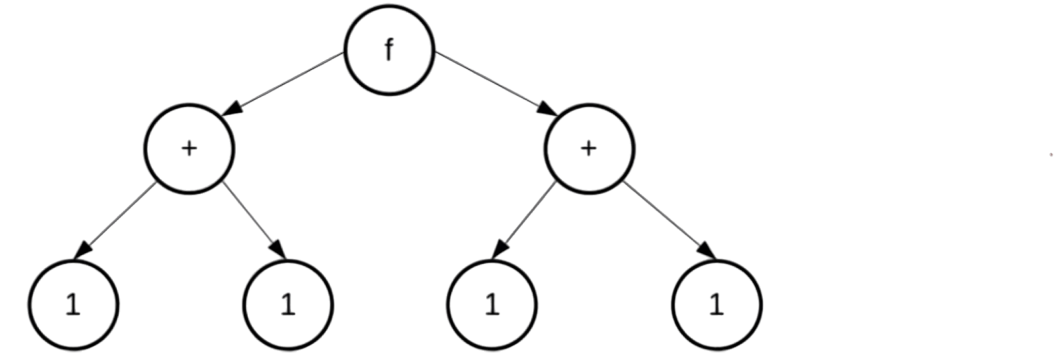
\includegraphics[width=0.5\textwidth]{latex/assets/graph-reduction.png}

To implement the concept of ``sharing'', each non-value vertex points to a placeholder vertex where the resulting value will be stored, which in turn points to the expression. Therefore, sharing is where two or more placeholder vertices point to the same expression.

\medskip
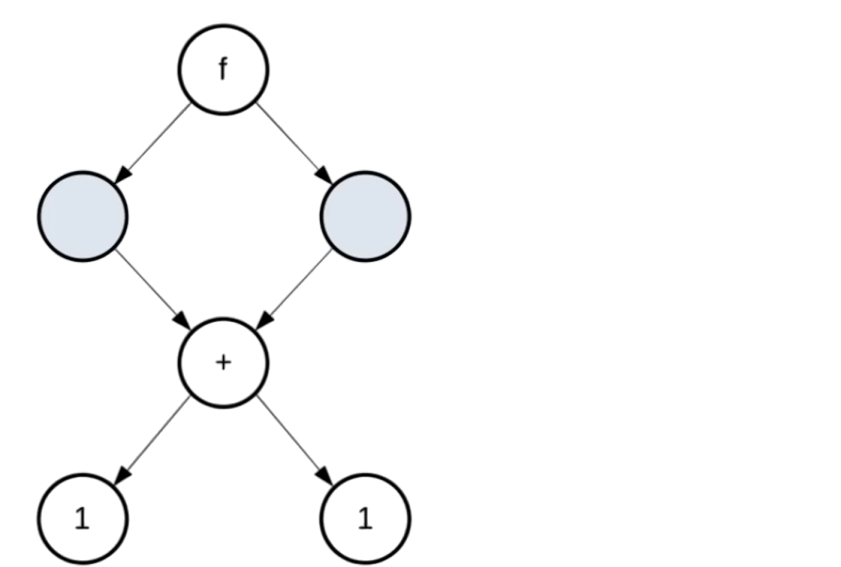
\includegraphics[width=0.5\textwidth]{latex/assets/graph-reduction-sharing.png}

\subsection{Sharing}
Possible due to lack of side effects, thunks which are equivalent need only be evaluated once and its value shared.
This is done by memoising evaluated thunks to avoid re-evaluation of equivalent thunks in the future.

\begin{lstlisting}[language=haskell]
(1 + 1) + 2 + (1 + 1)
= (2) + 2 + (2)
= (2) + 4
= 6
\end{lstlisting}

\subsection{Normal Form}
An expression is in a normal form if and only if it is fully evaluated (i.e. no further reductions can be applied).

Examples:
\begin{lstlisting}[language=haskell]
1 + 1 => 2
(1, 2+2) => (1, 4)
[True && False] => [False]
(\x -> x * 10) -- Already in normal form!
\end{lstlisting}

Note that the following are not in normal form:
\begin{itemize}
  \item \textit{Function definitions}. Expand the definition into a value.
  \begin{lstlisting}[language=haskell]
f x = ...
-- Becomes
f = \x -> ...\end{lstlisting}
  \item \textit{Top-level pattern matching}. Expand into a \texttt{case .. of ..} expression.
  \begin{lstlisting}[language=haskell]
f <p1> = <e1>
f <p2> = <e1>
-- Becomes
f = \x -> case x of
    p1 -> e1
    p2 -> e2
\end{lstlisting}
\end{itemize}

\subsubsection{Weak Head Normal Form}
An expression which is fully evaluated \textit{up to \textbf{at least}} the first data constructor. Values/equations in WHNF are:-
\begin{enumerate}
  \item Data constructors
  \item Built-in functions applied to too few arguments e.g. \texttt{(+ 2)}
  \item Lambda expressions
\end{enumerate}

\begin{lstlisting}[language=haskell]
1 + 1 => 2
(1, 2+2) -- In WHNF as values are inside a data constructor
[True && False] => _ : _ -- The values do not matter. Only the constructor '(:)' matters in WHNF.
\end{lstlisting}

The \texttt{seq} function is \textit{strict} in its first argument - it enforces its first argument to be evaluated to WHNF. This function is defined this way explicitly in GHC and is one of the only functions to do this.
\section{Variables}

Variables are name-bounded values. Variables in Haskell are immutable - they cannot be changed.

\begin{center}
  \texttt{\blue{name} = <value>}
\end{center}

Variable types are \textit{inferred}. To explicitly assign variables a type,

\begin{center}
  \texttt{\blue{name} :: \red{Type}}
\end{center}

In GHCI, the type of a symbol may be retriesed by \texttt{:t \blue{name}}.

\subsection{Local Name Binding}
Two methods are provided to bind a symbol to a value in a local scope: \texttt{let} and \texttt{where}. Each follow a ``main'' expression.

\subsubsection{\texttt{let}}
Syntax:
\begin{lstlisting}[language=haskell]
  let
    <symbol> = <expr>
    <symbol2> = <expr2>
    ...
  in
  <main_expr>
\end{lstlisting}

For example, re-define \texttt{\blue{in\_range}} as follows:

\begin{lstlisting}[language=haskell]
  in_range x min max =
    let
      in_lb = min <= x
      in_ub = max > x
    in
    in_lb && in_ub
\end{lstlisting}

\subsubsection{\texttt{where}}
Syntax:

\begin{lstlisting}[language=haskell]
  <main_expr>
  where
    <symbol> = <expr>
    <symbol2> = <expr2>
    ...
\end{lstlisting}

For example, re-define \texttt{\blue{in\_range}} as follows:

\begin{lstlisting}[language=haskell]
  in_range x min max = in_lb && in_ub
    where
      in_lb = min <= x
      in_ub = max > x
\end{lstlisting}
\section{Functions}

Functions are defined to map a value from an input set - the \textit{domain} - into an output set - \textit{the co-domain}. Every output of the function is contained in a subset of the co-domain, called the \textit{range}. \textbf{Pure} mathematical functions must be able to map every value from the domain, and each input value must map to only one output value.

In Haskell, occurences of functions are expanded into their RHS.

\subsection{Function Definition}

Functions are defined by providing its name, a list of arguments, and setting it equal to an expression.

\begin{center}
  \texttt{\textcolor{blue}{name} arg1 arg2 \ldots argn = <expr>}
\end{center}

The arguments may be set to constants, or may be given a name to accept a variable value.

The type of a function is specified by an arrow (\texttt{->}) seperated list of its argument types and its return type:

\begin{center}
  \texttt{\blue{func} :: \red{type$_1$} -> \red{type$_2$} -> \ldots -> \red{type$_n$} -> \red{type$_\text{return}$}}
\end{center}

For an example, take a function which returns the sum of the elements of an array:

\begin{lstlisting}[language=haskell]
  sum :: [a] -> Int -- Takes an array of arbitrary type and returns an integer
  sum [] = 0 -- Define the sum of an empty array to be zero
  sum (h:t) = h + sum t -- Define the sum of an array to be the head plus the sum of the tail
\end{lstlisting}

\subsubsection{Infix Functions}

A good example of infix functions are operators such as \texttt{+}. Functions which take two arguments may be writen between the arguments instead.

For example, say we had \texttt{\blue{add} a b = a + b}. Then \texttt{\blue{add} 5 7} and \texttt{5 \textasciigrave\blue{add}\textasciigrave 7} are equivalent.

To reference the function defined by an operator i.e. \texttt{+}, surround it with parenthesis i.e. \texttt{(+)}.

\subsubsection{Pattern Matching}

Parameters of functions may be matched against a pattern. Note that order matters: more specific patterns should be defined first, with general cases last.
\begin{itemize}
  \item Accept any value by using a symbol e.g. \texttt{f x = ...}.
  \item Accept a certain value e.g. \texttt{f 0 = ...}, \texttt{g [] = ...}
  \item List splicing using \texttt{(x:xs)} where \texttt{x} is the head, \texttt{xs} is the tail.
  \item Tuple unpacking e.g. \texttt{(Int,Int)} could be unpacked using \texttt{(x,y)}.
  \item Accept and extract a custom types. E.g., say we had \texttt{\blue{type} Pos = (Int, Int)}, we would define \texttt{getX (x, y) = x}.
  \item Accept and extract a custom datatype. E.g., say we had \texttt{\blue{data} Num = Zero | Succ Num}. We could then define \texttt{f Zero = ...} and \texttt{f (Succ n) = ...}.
\end{itemize}

Pattern matching may also be done using \texttt{\blue{case} ... \blue{of} ...} construct.

\subsection{Function Application}

A function is applied (called) to some arguments as follows:

\begin{center}
  \texttt{\blue{name} arg1 arg2 \ldots argn}
\end{center}

For example, consider the function \texttt{\blue{in\_range} x min max = x >= min \&\& x < max}, an implementation of $x \in [min, max)$.

Then, \texttt{\blue{in\_range} 3 0 5} would evaluate to True, but \texttt{\blue{in\_range} 5 0 5} would evaluate to False.

\subsection{Recursion}
Recursion is the process of a function calling itself. Recursion requires a \textit{base case} to stop the function recursing indefinitely.

There are many ways to implement recursion, which will be demonstrated using the \textit{factorial}, defined as
\[n! = n \cdot (n - 1) \cdot \ldots \cdot 1 = \prod_{k = 1}^{n} k\]

\subsubsection{Defined Base Case}
We can hard-code the case where the function is called with the base case:

\begin{lstlisting}[language=haskell]
  fac 1 = 1
  fac n = n * fib (n-1) 
\end{lstlisting}

\subsubsection{If-Else Expression}
We can use the if-else expression:

\begin{center}
  \texttt{\blue{if} <expr> \blue{then} <ifTrue> \blue{else} <ifFalse>}
\end{center}

For example,

\begin{lstlisting}[language=haskell]
  fac n = if n <= 1 then 1 else n * fac (n-1)
\end{lstlisting}

\subsubsection{Guards}
Guards are similar to piece-wise functions.

\begin{lstlisting}[language=haskell]
<main_expr>
  | <expr> = <value>
  | <expr2> = <value2>
  ...
  | otherwise = <default_value>
\end{lstlisting}
Where \texttt{<expr>} is a boolean expression. If \texttt{<expr>} is matches, then \texttt{<value>} will be returned. If none is matched, the \texttt{\blue{otherwise}} is returned.

For example,

\begin{lstlisting}[language=haskell]
  fac n =
    | n <= 1    = 1
    | otherwise = n * fac (n-1)
\end{lstlisting}

\subsubsection{Accumulators}
In this example, we define an auxiliary function \texttt{\blue{aux}} inside \texttt{\blue{fac}} to calculate the the factorial

\begin{lstlisting}[language=haskell]
  fac n = aux n 1
    where
      aux n acc
        | n <= 1    = acc
        | otherwise = aux (n-1) (n*acc)
\end{lstlisting}

This is called \textit{tail recursion}. This is because the final result of \texttt{\blue{aux}} is the result we want, meaning that it is much more memory efficient. A good compiler could even unwind this into a non-recursive imperative approach using a loop. (For more insight, see \url{https://www.youtube.com/watch?v=_JtPhF8MshA}.)

Normal recursion (using an above definition of \texttt{\blue{fac}}):
\begin{verbatim}
fac 4
= 4 * fac 3
= 4 * (3 * fac 2)
= 4 * (3 * (2 * fac 1))
= 4 * (3 * (2 * 1))
= 4 * (3 * 2)
= 4 * 6
= 24
\end{verbatim}

Tail recursion (using the definition in this sub-section):
\begin{verbatim}
fac 4
= aux 3 4
= aux 2 12
= aux 1 24
= 24
\end{verbatim}

\subsection{Lambdas}
Syntax:
\begin{center}
  \texttt{(\blue{\symbol{92}}<args> -> <expr>)}
\end{center}

Some examples:
\begin{itemize}
  \item \texttt{(\symbol{92}x -> x+1) 2} returns \texttt{3}.
  \item \texttt{(\symbol{92}x y z -> x+y+z) 1 2 3} returns \texttt{6}.
\end{itemize}
Lambdas may be bound to names.

\subsection{Higher Order Functions}
Higher order functions are functions that take other functions as arguments.

For example, a function which takes another function and applies it to an argument:
\begin{lstlisting}[language=haskell]
  app :: (a -> b) -> a -> b
  app f x = f x
\end{lstlisting}
A synonym of such a function is the dollar (\texttt{\$}) operator: \texttt{(\$) :: (a -> b) -> a -> b}.

\subsubsection{Useful Higher Order Functions}
\begin{itemize}
  \item \texttt{\blue{map} :: (a -> b) -> [a] -> [b]} applies a function to every element on an array.
  \[L' = \{f(x) : x \in L\}\]
  
  Example: \texttt{\blue{map} (\symbol{92}x -> x\string^2) [1,2,3]} returns \texttt{[1,4,9]}.
  \item \texttt{\blue{filter} :: (a -> \red{Bool}) -> [a] -> [a]} filters the list on a predicate.
  \[L' = \{x \in L : P(x)\}\]
  
  Example: \texttt{\blue{filter} (\symbol{92}x -> mod x 2 == 0) [1,2,3,4,5]} returns \texttt{[2,4]}.
  \item \texttt{\blue{fold} :: (a -> b -> b) -> b -> [a] -> b} processes a list with some function to produce a single value, starting at a given value.
  
  In Haskell, \texttt{\blue{fold}} doesn't exist, but rather \texttt{\blue{foldr}} and \texttt{\blue{foldl}} which start folding at either end of the list respectively.
  \[\texttt{\blue{foldr}}\; (op)\; a\; [x_1, x_2, \ldots, x_n] = x_1\; (op)\; x_2\; (op)\; \ldots\; (op)\; x_n\; (op)\; a\]
  \[\texttt{\blue{foldl}}\; (op)\; a\; [x_1, x_2, \ldots, x_n] = a\; (op)\; x_n\; (op)\; x_{n-1}\; (op)\; \ldots\; (op)\; x_1\]

  Example: \texttt{\blue{foldr} (+) 0 [1,2,3,4,5]} returns \texttt{15}.
\end{itemize}

\subsection{Currying}
The principle behind currying is that given
\begin{center}
  \texttt{\blue{f} :: a -> b -> c -> d}
\end{center}
We could re-write this as
\begin{center}
  \texttt{\blue{f'} :: a -> (b -> (c -> d))}
\end{center}

For example, one could define a function \texttt{\blue{add}} in multiple ways:
\begin{lstlisting}[language=haskell]
  add x y = x + y
  add x = (\y -> x + y)
  add = (\x -> (\y -> x + y))
\end{lstlisting}

\subsection{Currying \& Uncurrying}
Let's illustrate these terms by defining functions,

\begin{center}
  \texttt{\blue{curry} :: ((a,b) -> c) -> a -> b -> c}

  \texttt{\blue{curry} f x y = f (x,y)}
\end{center}

\begin{center}
  \texttt{\blue{uncurry} :: (a -> b -> c) -> (a,b) -> c}

  \texttt{\blue{uncurry} f (x,y) = f x y}
\end{center}

\subsubsection{Partial Function Application}
Using the last definition of \texttt{\blue{add}}, consider the result of \texttt{\blue{add} 1}. This would be a new function; \texttt{\blue{add} 1 :: \red{Int} -> \red{Int}}. This is known as a \textit{section}.

A good example would be using \texttt{\blue{map}}.
\begin{center}
  \texttt{\blue{doubleList} = \blue{map} (\symbol{92}x -> x * 2)}
\end{center}

\subsection{Function Composition}
Function composition is a way to combine functions. For this, we use the dot (\texttt{.}) operator.
\begin{center}
  \texttt{(.) :: (b -> c) -> (a -> b) -> (a -> c)}
\end{center}
Then, \texttt{(f.g)} is equivalent to \texttt{(\blue{\symbol{92}}x -> f (g x))}.

For example, all three definitions of \texttt{\blue{descSort}} are equivalent:
\begin{lstlisting}[language=haskell]
  descSort = reverse . sort
  descSort = (\x -> reverse (sort x))
  descSort = reverse (sort x)
\end{lstlisting}
\section{Types}

Every expression in Haskell has a type. Types are inferred, even when given explicitly.

Types always begin with an UPPERCASE letter.

The cardinality of a type is how many \textit{states} the data type could hold. Polymorphic types have no cardinality.

\subsection{Variable Types}

\begin{center}
  \texttt{var :: \red{type}}
\end{center}

\subsubsection{Lists}

To define a list of a \texttt{\red{type}}, one would write \texttt{[\red{type}]}. This may be nested.

\subsection{Function Types}

\begin{center}
  \texttt{func :: \red{type1} -> ... -> \red{typeN} -> \red{ret\_type}}
\end{center}

Where the function \texttt{func} takes $n$ arguments of types \texttt{\red{type1}, ..., \red{typeN}} and returns \texttt{\red{ret\_type}}.

\subsubsection{Type Variables}

Type variables may be used where any type would be permissable and must be lowercase. For example,

\begin{center}
  \texttt{id :: a -> a}

  \texttt{id x = x}
\end{center}

This is called ``parametric polymorphism''.

\subsection{Type Aliasing}
This doesn't define a new datatype, but rather an alias for another type.
\begin{center}
  \texttt{\blue{type} Pos = \red{type}}
\end{center}

A common example is using a tuple e.g. \texttt{\blue{type} Pos = (\red{Int}, \red{Int})}. The type name need not be stated in pattern matching.

\subsection{Type Classes}
Type classes may be used to restrict the types a polymorphic function may take. This is useful if we would like to use features in a polymorphic function that may only be available to certain types. For a type to be a member of a type class, it must implement all of the required methods.

To impose a constraint on variable \texttt{a} in a function \texttt{f}: \texttt{f :: (\texttt<TypeClass> a, ...) => ...}. This is called ``ad-hoc polymorphism''.

\subsubsection{Definition}
A type class definition begins with

\texttt{\blue{class} <Name> <var> \blue{where}}

Below is a list of function declarations. For a type to be a member of \texttt{<Name>}, it must implement all of these functions.

\subsubsection{Implementation}
To define a new type which belongs to a type class:
\texttt{\blue{instance} <TypeClass> <TypeName> \blue{where}}

Where below this is a list of function definitions.

\subsubsection{Common Type Classes}
Common type classes include:
\begin{itemize}
  \item \texttt{\red{Eq}} -- types which may be compared i.e. \texttt{(==)} is defined;
  \item \texttt{\red{Num}} -- numeric types, gives us access to standard mathematical operations i.e. \texttt{(+), (-), (*), abs, ...} are defined;
  \item \texttt{\red{Ord}} -- types which may be ordered, imposes a total ordering i.e. \texttt{(<), (>), (<=)} are defined;
  \item \texttt{\red{Read}} -- types which may be converted from a string i.e. \texttt{read} is defined;
  \item \texttt{\red{Show}} -- types which may be converted to a string i.e. \texttt{show} is defined;
  \item \texttt{\red{Integral}} -- types which are integer-like i.e. \texttt{div, ...} is defined;
  \item \texttt{\red{Floating}} -- types which are float-like i.e. \texttt{(/), ...} is defined;
  \item \texttt{\red{Enum}} -- types which may be enumerated i.e. \texttt{succ, pred, ...} are defined;
\end{itemize}

\textit{N.B. for information on complex type classes, see Type Class section}

\subsubsection{Instances}
Intances allow us to write functions which make use of type classes. Syntax:

\texttt{\red{instance} (<constraints>) => <typeClass> <value> \red{where}} followed by a list of function definitions.

\subsubsection{Derivation}
The \texttt{\blue{deriving}} keyword can be used to automatically generate implementations for the given type class(es).

Syntax: \texttt{\blue{data} <Name> = \ldots \blue{deriving} (<Class1>, \ldots)}

Example: \texttt{\blue{data} Shape = Circle Int | Rect Int Int \blue{deriving} Show}. Then, \texttt{\blue{print} (Circle 5)} $\rightarrow$ \texttt{Circle 5}.

\subsection{Defining Datatypes}
The \blue{data} keyword is used to define a new datatype; unlike the above, these are entirely custom.

This may be done using the \texttt{data} keyword:
\begin{center}
  \texttt{\blue{data} Name = \red{Constructor1} [<args>] | \ldots}
\end{center}
where \texttt{<args>} are the \textit{types} of each argument, not literals.

Constructors are either plain values, or functions which take \texttt{args} and return the datatype.

Data consturctors can include polymorphism by including type variables after \texttt{<Name>} e.g. \texttt{\blue{data} Maybe a = Nothing | Just a}.

\subsubsection{Examples}
\begin{itemize}
  \item \url{rock-paper-scissors.hs} -- A basic example revolving around Rock-Paper-Scissors;
  \item \url{expr.hs} -- A program to build and evaluate expressions;
  \item \url{tree.hs} -- A representation of a tree structure;
  \item \url{nat-num.hs} -- A definition of natural numbers using the successor function;
\end{itemize}

\subsection{Records}
Records allow data to be stored with an associated name.

Syntax:
\begin{center}
  \texttt{\blue{data} <Name> = <Name> \{ <field> :: <type>, \ldots \}}
\end{center}
This will automatically generate functions \texttt{<field> :: <Name> -> <type>} to extract said properties. This has the side-effect that field names must be globally unique.

\subsubsection{Multiple Constructors}
Note that records may also have mutliple constructors,

\texttt{\blue{data} Point = D2 \{ x :: \red{Int}, y :: \red{Int} \} | D3 \{ x :: \red{Int}, y :: \red{Int}, z :: \red{Int} \}}

Duplicate field names in this context is OK.

This will generate functions \texttt{x}, \texttt{y} and \texttt{z} all with the signature \texttt{x/y/z :: Point -> \red{Int}}. Both \texttt{x} and \texttt{y} will work on either \texttt{D2} or \texttt{D3}, but applying \texttt{z} to \texttt{D2} will throw an exception.

For an example, see \url{code/vector.hs}.
\section{Useful Types}
This section will list some common, useful types which should be known.

\subsection{Maybe}
The \texttt{Maybe} type is incredibly useful, as it can be used to represent the \textit{absence} of a value. This is useful when our function is passed invalid data, for example.

If it defined as: \texttt{\blue{data} Maybe a = Nothing | Just a}

\paragraph{Functions}
Found inside \texttt{Data.Maybe}.
\begin{itemize}
  \item \texttt{isJust :: Maybe a -> \red{Bool}} -- returns if the passed \texttt{Maybe} is a \texttt{Just} value;
  \item \texttt{fromMaybe :: a -> Maybe a -> a} -- returns the \texttt{Just} value if a value is present, else returns the default value;
  \item \texttt{fromJust :: Maybe a -> a} -- returns the \texttt{Just} value, or throws an exception if recieved \texttt{Nothing};
  \item \texttt{catMaybes :: [Maybe a] -> [a]} -- returns a list containing all the \texttt{Just} values.
  \item \texttt{mapMaybe :: (a -> Maybe b) -> [a] -> [b]} -- maps a function over a list of \texttt{Maybe}s, discarding any \texttt{Nothing}s;
  \item \texttt{maybe :: b -> (a -> b) -> Maybe a -> b} -- takes a maybe. If \texttt{Just}, applies a function and returns. Else, returns a default;
\end{itemize}

\subsection{Either}
The \texttt{Either} type can be used to represent a union of types -- a value which is either one type, or another.

It is defined as \texttt{\blue{data} Either a b = Left a $\mid$ Right b}

\paragraph{Functions}
Found inside \texttt{Data.Either}.
\begin{itemize}
  \item \texttt{lefts :: [Either a b] -> [a]} -- returns an array of left-hand side values;
  \item \texttt{rights :: [Either a b] -> [b]} -- returns an array of right-hand side values;
  \item \texttt{isLeft :: Either a b -> \red{Bool}} -- returns whether the provided value is a left-hand side value;
  \item \texttt{isRight :: Either a b -> \red{Bool}} -- returns whether the provided value is a right-hand side value;
  \item \texttt{fromLeft :: a -> Either a b -> a} -- returns the left-hand side value if a \texttt{Left} is provided, else returns a default;
  \item \texttt{fromRight :: n -> Either a b -> n} -- returns the right-hand side value if a \texttt{Right} is provided, else returns a default;
  \item \texttt{either :: (a -> c) -> (b -> c) -> Either a b -> c} -- processes the left- or right-hand value in the \texttt{Either} as per the given functions;
  \item \texttt{partitionEithers :: [Either a b] -> ([a],[b])} -- traverses the list, placing and \texttt{Left} values in one list and any \texttt{Right} values in another;
\end{itemize}

\paragraph{Use -- Error Handling}
\texttt{Either} can be used in place of \texttt{Maybe} for error handling.

\texttt{Left} can represent a correct input/output with \texttt{Right} holding the incorrect value.
\section{Collections}

Haskell has two collections: lists, and tuples.

\subsection{Lists}
A \textit{mutable} collection of elements of the \textit{same type}. Every elements has an ordinal.

A list of type \texttt{\red{type}} has the given type signature
\begin{center}
  \texttt{\blue{name} :: [\red{type}]}
\end{center}

\subsubsection{Construction}
A list may be greated by the following constructor:
\begin{itemize}
  \item Using square brackets: \texttt{[$x_1$, $x_2$, \ldots, $x_n$]}
  \item Using the prepend opeator: \texttt{$x_1:x_2:\ldots:x_n:$[]}. With the syntax of \texttt{x:list}, it prepends \texttt{x} to the list \texttt{list}.
\end{itemize}

\subsubsection{Pre-defined functions}
Many pre-defined functions for lists are defined in the \texttt{Data.List} module.

\paragraph{General Functions} These functions work on a list of any type, namely \texttt{[a]}.
\begin{itemize}
  \item \texttt{\blue{head} <list>}. This function returns the head ($x_1$) of the list. Example: \texttt{\blue{head} [1,2,3]} returns \texttt{1}.
  \item \texttt{\blue{tail} <list>}. This function returns the tail of the list. Example: \texttt{\blue{tail} [1,2,3]} returns \texttt{[2,3]}.
  \item \texttt{\blue{length} <list>}. This function returns the length of the list. Example: \texttt{\blue{length} [1,2,3]} returns \texttt{3}.
  \item \texttt{\blue{init} <list>}. This function returns the list without the last element. Example: \texttt{\blue{init} [1,2,3]} returns \texttt{[1,2]}.
  \item \texttt{\blue{null} <list>}. This function returns whether the list is empty. Example: \texttt{\blue{null} [1,2,3]} returns \texttt{\red{False}}.
  \item \texttt{\blue{take} <n> <list>}. This function returns a list of the first $n$ elements of the list. Example: \texttt{\blue{take} 2 [1,2,3,4,5]} returns \texttt{[1,2]}.
  \item \texttt{\blue{drop} <n> <list>}. This function returns a list excluding the first $n$ elements of the list. Example: \texttt{\blue{drop} 2 [1,2,3,4,5]} returns \texttt{[3,4,5]}.
\end{itemize}

\paragraph{Boolean Functions} These functions are of the type \texttt{\blue{fn} :: [\red{Bool}] -> \red{Bool}}
\begin{itemize}
  \item \texttt{\blue{and} <list>}. This functions returns \texttt{\red{True}} if every elements in \texttt{<list>} is \texttt{\red{True}}.
  \item \texttt{\blue{or} <list>}. This functions returns \texttt{\red{True}} if at least one element in \texttt{<list>} is \texttt{\red{True}}.
\end{itemize}

\subsubsection{List Comprehension}
List comprehension can be used to transform one or more lists according to a predicate. Syntax:
\begin{center}
  \texttt{[ <gen> | <elem> <- <list>, \ldots, <guard>, \ldots ]}
\end{center}
Examples:
\begin{itemize}
  \item \texttt{[ 2*x | x <- [1,2,3] ]} generates \texttt{[2,4,6]}
  \item \texttt{[ x\^{}2 | x <- [1,2,3], x > 1 ]} generates \texttt{[4,9]}
  \item \texttt{[ (x,y) | x <- [1,2,3], y <- [`a',`b'] ]} generates
  
  \texttt{[(1,`a'),(1,`b'),(2,`a'),(2,`b'),(3,`a'),(3,`b')]}
\end{itemize}

\subsubsection{Ranges}
Generate ranges in Haskell using the ellipse \text{..}:
\begin{center}
  \texttt{[<start> .. <end>]}
\end{center}

E.g. \texttt{[1 .. 5] = [1,2,3,4,5]}. \texttt{<end>} may be omitted to generate an infinite list e.g. \texttt{[1 ..] = [1,2,3,...]}

\subsection{Tuples}
An \textit{immutable} collection of elements of \textit{different types}.

A tuple has the signature
\begin{center}
  \texttt{(x,y,...) :: (type$_x$, type$_y$, ...)}
\end{center}
\section{Kinds}

The types of \textit{types} and \textit{type constructors} are called \textit{kinds}.

A kind signature is denoted by \texttt{::.}. The number of \textit{kinds} correspond to the number of type parameters a type constructor takes.
\begin{itemize}
  \item Types which take no type parameters are of kind \texttt{*} (``\textit{type}'').
  \begin{itemize}
    \item \texttt{\red{Bool} :: *}
    \item \texttt{\red{String} :: *}
    \item \texttt{Maybe :: * -> *}
  \end{itemize}
  \item When we apply a type parameter, one of the parameters is consumed in the kind
  \begin{itemize}
    \item \texttt{Maybe \red{Int} :: *}
  \end{itemize}
\end{itemize}
\section{Modules}

In Haskell, each file is a module. Hence, each file (other than the entry file) must begin with a module declaration:

\begin{center}
  \texttt{\blue{module} \textit{filename} [(n1, n2, ...)] \blue{where}}
\end{center}

By default, every symbol is exported. If \texttt{(n1, n2, ...)} is included, only symbols \texttt{n1}, \texttt{n2} etc. are exported.

\subsection{Importing}

To import a module, use an import statement:

\begin{center}
  \texttt{\blue{import} \textit{module} [(n1, n2, ...)]}
\end{center}

By default, every symbol exported by \texttt{module} is imported. If \texttt{(n1, n2, ...)} is included, only symbols \texttt{n1}, \texttt{n2} etc. are imported.

To import \url{Animals.hs} one would write \texttt{\blue{import} Animals}.
To import \url{Farm/Tractor.hs} one would write \texttt{\blue{import} Farm.Tractor}.

Once imported, symbols may be used freely. For example, if the function \texttt{double} is imported, to reference it we would write \texttt{double}. However, if two different definitions for \texttt{double} are imported, we must use its full name e.g. \texttt{Module.double}.

\subsubsection{Qualified Imports}

Syntax:

\begin{center}
  \texttt{\blue{import qualified} \textit{module} [(...)]}
\end{center}

This forces the module name to precede any symbols imported. In the example above, \texttt{Module.double} \textbf{must} be used.

\subsubsection{Aliased Imports}

Syntax:

\begin{center}
  \texttt{\blue{import} \textit{module} [(...)] \blue{as} \textit{alias}}
\end{center}

Using the above example, now, instead of writing \texttt{Module.double} one would now write \texttt{Alias.double}.

\subsubsection{Import Hiding}
The \texttt{\blue{hiding}} keyword can be used to omit imports.
E.g. \texttt{\blue{import} Prelude \texttt{hiding} (map)} would import every function from \texttt{Prelude} but omit \texttt{map}.
\section{Type Classes}
This section covers more complex type classes. For basics, see \texttt{Types -> Type Classes}.

\subsection{Semigroups}
A type is a Semigroup if there exists some function which, when two values from the group are combined, that value is also in the Semigroup.

\begin{lstlisting}[language=haskell]
class Semigroup a where
  (<>) :: a -> a -> a

infixr 6 <>
\end{lstlisting}

This diamond operator must be \textbf{associative}:
\begin{lstlisting}[language=haskell]
x <> (y <> z) == (x <> y) <> z
\end{lstlisting}

\subsection{Monoid}
A Monoid is an extension of a Semigroup, adding an identity element.
\begin{lstlisting}[language=haskell]
class Semigroup a => Monoid a where
  mempty :: a

  -- Optional functions
  mappend :: a -> a -> a
  mappend = (<>)

  mconcat :: [a] -> a
  mconcat = foldr mappend mempty
\end{lstlisting}

\texttt{mempty} must be an identity element for the Semigroup. Therefore, it must obey:
\begin{lstlisting}[language=haskell]
x <> mempty == x
mempty <> x == x
\end{lstlisting}

\subsubsection{Multiple Monoids}
A type may have multiple Monoid implementations (i.e. multiple viable operators exist which satisfy Monoidal conditions).

For example, take numerical types:
\begin{lstlisting}[language=haskell]
newtype Sum n = Sum { getSum :: n }
instance Num a => Semigroup (Sum a) where
  (<>) = (+)
instance Num a => Monoid (Sum a) where
  mempty = 0


newtype Product n = Product { getProduct :: n }
instance Num a => Semigroup (Product a) where
  (<>) = (*)
instance Num a => Monoid (Product a) where
  mempty = 1

\end{lstlisting}

\subsection{Foldable}
A Foldable datatype is one which may be reduced to a single value i.e. folded in on itself.
\begin{lstlisting}[language=haskell]
class Foldable t where
  foldr :: (a -> b -> b) -> b -> t a -> b
\end{lstlisting}

\subsection{Functors}
A Functor is a type class which may have an operation mapped over it.

\begin{lstlisting}[language=haskell]
class Functor f where
  fmap :: (a -> b) -> f a -> f b -- Infix symbol is <$>

  -- The following functions are optional
  (<$) :: a -> f b -> f a
  (<$) = fmap . const
\end{lstlisting}

A Functor instance must obery the following laws:
\begin{itemize}
  \item The mapping must preserver the structure of the arguments.
  \item \textbf{Identity}: \begin{lstlisting}[language=haskell]
fmap id == id\end{lstlisting}
  \item \textbf{Distributive over Composition}: \begin{lstlisting}[language=haskell]
fmap (f . g) == fmap f . fmap g\end{lstlisting}
\end{itemize}

\subsubsection{Fmap}
\texttt{fmap} allows a function to be mapped over a structure without the internal structure of the Functor changing.

\textbf{Example}:
\begin{lstlisting}[language=haskell]
data Tree a = Leaf a | Node (Tree a) a (Tree a)

instance Functor Tree where
  fmap f (Leaf a) = Leaf (f a)
  fmap f (Node a b c) = Node (fmap f a) (f b) (fmap f c)
\end{lstlisting}

\subsection{Applicatives}
Applicatives are Functors with more and better functionality, with \texttt{<*>} essentially \textit{injecting} a value into a wrapped function, and \texttt{pure} allowing easy construction of an applicative.

\begin{lstlisting}[language=haskell]
class Functor f => Applicative f where
  pure :: a -> f a
  (<*>) :: f (a -> b) -> f a -> f b

  -- Optional functions
  (*>) :: f a -> f b -> f b
  a *> b = b
  (<*) :: f a -> f b -> f a
  a <* b = a
\end{lstlisting}

An Applicative must obey the following laws:
\begin{itemize}
  \item \textbf{Identity}: \begin{lstlisting}[language=haskell]
pure id <*> v == v\end{lstlisting}
  \item \textbf{Homomorphism}: \begin{lstlisting}[language=haskell]
pure f <*> pure x == pure (f x)\end{lstlisting}
  \item \textbf{Interchange}: \begin{lstlisting}[language=haskell]
u <*> pure y == pure (\$ y) <*> u\end{lstlisting}
  \item \textbf{Composition}: \begin{lstlisting}[language=haskell]
pure (.) <*> u <*> v <*> w == u <*> (v <*> w)\end{lstlisting}
\end{itemize}

\subsection{Monads}
A Monad allows the transformation of a value into a Monad via a function.

\begin{lstlisting}[language=haskell]
class Applicative m => Monad m where
  (>>=) :: m a -> (a -> m b) -> m b -- "Bind"

  -- Optional functions
  (>>) :: m a -> m b -> m b -- "Then"
  a >> b = a >>= \x -> b

  return :: a -> m a
  return = pure
\end{lstlisting}

Any implementation must abide by these laws:
\begin{itemize}
  \item \textbf{Left identity}: \begin{lstlisting}[language=haskell]
return a >>= h == h a\end{lstlisting}
  \item \textbf{Right identity}: \begin{lstlisting}[language=haskell]
m >>= return == m\end{lstlisting}
  \item \textbf{Associativity}: \begin{lstlisting}[language=haskell]
(m >>= g) >>= h == m >>= (\x -> g x >>= h)\end{lstlisting}
\end{itemize}

\subsubsection{Bind}
\bordertext{\texttt{(>>=) :: \red{Monad} m => m a -> (a -> m b) -> m b}}
This function takes a monad and a function which takes a raw value and returns a new monad, and returns another new monad.

When implemented, then, we may vary the action taken depending on the value of the provided monad, such as returning a default value -- this is what \texttt{(>>=)} does with \texttt{Maybe}, as shown below: 

\textbf{Example}:
\begin{lstlisting}[language=haskell]
  add :: Num a => Maybe a -> Maybe a -> Maybe a
  add mx my = mx >>= (\x -> my >>= (\y -> Just (x + y)))

  -- Then addition works as expected
  add (Just 1) (Just 2) -- => Just 3
  -- And if either one of the arguments is Nothing, it returns Nothing
  add Nothing (Just ?) -- => Nothing
\end{lstlisting}

\subsubsection{Then}
\bordertext{\texttt{(>>) :: \red{Monad} m => m a -> m b -> m a}}

This function discards the second monad given to it. \texttt{m >> n} is equivalent to \texttt{m >>= \symbol{92}\_ -> n}.

``Then'' can be though of wanting to carry out an action but not caring what the result is.

\subsubsection{Return}
\bordertext{\texttt{return :: \red{Monad} m => a -> m a}}

Return wraps a monad around a raw value.

Using the example from the Bind section, we could substitute the explicit \texttt{Just} with the more general \texttt{return}. Now, this would theoretically work with any appropriately-defined monad.

\begin{lstlisting}[language=haskell]
  add mx my = mx >>= (\x -> my >>= (\y -> return (x + y)))
\end{lstlisting}

\subsubsection{Fail}
\bordertext{\texttt{fail :: \red{Monad} m => \red{String} -> m a}}

Fail is intended to be called when something goes wrong. The default implementation is to call \texttt{error} (i.e. error out of the program), but it may be implemented so that certain errors may be handled and return an appropriate monad as a response.

\subsubsection{``do'' Syntax}

Chaining together applications of \texttt{(>>=)}, \texttt{(>>)} and lambda functions can get tedious; that's where the syntactic sugar ``do'' expression comes in.

The ``statements'' inside of \texttt{do} are executed in order, and if one ``statement'' fails this will be propagated through.

\begin{itemize}
  \item \textbf{Bind} \begin{lstlisting}[language=haskell]
    m >>= \x -> ...
    -- Becomes
    do
      x <- m
      ...
  \end{lstlisting}
  \item \textbf{Then} \begin{lstlisting}[language=haskell]
    m >> ...
    -- Becomes
    do
      m
      ...
  \end{lstlisting}
\end{itemize}

\textbf{Example}:
\begin{lstlisting}[language=haskell]
  -- Re-writing the above definition of 'add'
  add mx my = do
    x <- mx
    y <- my
    return $ x + y
\end{lstlisting}

\subsubsection{Kleisli-Composition}
This operator, denoted \texttt{>=>}, acts as a Monad composition operator. It is defined in \texttt{Control.Monad} as so
\begin{lstlisting}[language=haskell]
infixr 1 >=>
(>=>) :: Monad m => (a -> m b) -> (b -> m c) -> a -> m c
f >=> g = \x -> f x >>= g
\end{lstlisting}

\section{I/O}

I/O produces an issue with Haskell as I/O functions aren't \textit{pure}.

\subsection{The \texttt{IO} Type}
All I/O functions in Haskell have the following type: \texttt{IO \red{<value>}}.

This special type holds a given I/O action. When the \texttt{IO} value is used, the stored action will be carried out, and \texttt{IO \red{<value>}} is returned.

For example, in GHCI

\texttt{> hi = putStrLn "Hello, World!"}

\texttt{> hw}

\texttt{Hello, World!}

Notice how nothing was outputted until the \texttt{IO} value was used. Note that \texttt{hw} may be used mutliple times.

\subsection{Input}
\begin{itemize}
  \item \texttt{getLine :: IO \red{String}} -- retrieves a line of input from STDIN;
  \item \texttt{readLn :: Read a => IO a} -- retrieves a line of input from STDIN, reading it as specified by \texttt{a};
\end{itemize}

\subsection{Output}
\begin{itemize}
  \item \texttt{putStr :: \red{String} -> IO ()} -- puts the given string to STDOUT;
  \item \texttt{putStrLn :: \red{String} -> IO ()} -- puts the given string to STDOUT on a new line;
  \item \texttt{print :: Show a => a -> IO ()} -- essentially the same as \texttt{putStrLn . show};
\end{itemize}

\subsection{Extracting \texttt{<value>}}
\texttt{IO} is a \textit{monad}, and should be extracted as such.
\begin{lstlisting}[language=haskell]
greet :: IO ()
greet = do
  putStrLn "What is your name?"
  name <- getLine
  putStrLn $ "Hello, " ++ name ++ "!"
\end{lstlisting}

You can only extract values from \texttt{IO} inside of another \texttt{IO} action.

For a more complex example, see \url{code/IO.hs}.

\subsection{Environment}
The following functions are defined in \texttt{System.Environment}.

\subsubsection{Command-Line Arguments}
Command-line arguments are arguments passed to the executable e.g. \texttt{./prog.exe arg1 arg2 ...}

These can be accessed via \texttt{getArgs :: IO [\red{String}]}

Note, the program name ``\texttt{prog.exe}'' is ommited; this can be access via \texttt{getProgName :: IO String}

\subsubsection{Environment Variables}
The function \texttt{getEnvironment :: IO [(String, String)]} gets a list of all environment variables in name-value pairs.

To get only one variable, the function \texttt{lookupEnv :: String -> IO (Maybe String)} returns the value of an environment variable.

The function \texttt{withArgs :: [String] -> IO a -> IO a} loads sets the environment variables inside an IO action.

\subsubsection{Error Handling}
Defined in \texttt{System.Exit}

\begin{itemize}
  \item \texttt{exitWith :: ExitCode -> IO a} exits the program with the provided exit code (\texttt{ExitCode = ExitSuccess | ExitFailure Int});
  \item \texttt{exitSuccess :: IO a} exits the program with exit code of success;
  \item \texttt{exitFailure :: IO a} exits the program with exit code of failure (1);
  \item \texttt{die :: String -> IO a} prints the given message, then exits the program with exit code of failure (1);
\end{itemize}

\subsection{Files}
The symbols \texttt{stdout :: Handle} and \texttt{stdin :: Handle} are handles to the process' input/output streams. I/O functions defined above use the following functions with these handles provided.

\begin{itemize}
  \item \texttt{readFile :: FilePath -> IO \red{String}} -- reads contents of the file
  \item \texttt{writeFile :: FilePath -> \red{String} -> IO ()} -- writes to the file (overwrites contents if exists)
  \item \texttt{appendFile :: FilePath -> \red{String} -> IO ()} -- appends to the file
  \item \texttt{renameFile :: FilePath -> FilePath -> IO ()} -- renamed the given file to the second argument
  \item \texttt{deleteFile :: \red{String} -> IO ()} -- deletes the given file
\end{itemize}

Alternatively, you can use file handles.
\begin{itemize}
  \item \texttt{openFile :: FilePath -> IOMode -> IO Handle} -- Open a file in the given mode.
  
  \texttt{\blue{data} IOMode = ReadMode | WriteMode | AppendMode | ReadWriteMode}
  \item \texttt{hGetContents :: Handle -> IO String} -- Get contents of the file
  \item \texttt{hPutStr :: Handle -> \red{String} -> IO ()} -- writes the given string to the file
  \item \texttt{hPrint :: Show a => Handle -> a -> IO ()} -- converts \texttt{a} to a string and write to the file
  \item \texttt{hClose :: Handle -> IO ()} -- Close the given handle
  \item \texttt{withFile :: FilePath -> IOMode -> (Handle -> IO a) -> IO a} -- opens a file, processes it according to the function, then closes it
\end{itemize}

\section{Category Theory}
This section will contain a brief look into category theory and how it applies to Haskell. Various concepts such as Applicatives and Monads are discussed mathematically; for a more haskell-focused approach, see chapter \texttt{Type Classes}.

A category is a collection of \textit{objects} and \textit{arrows}. Arrows acts as pathways between objects.
\begin{itemize}
  \item $A \to B$ is a \textit{morphism} from $A$ to $B$.
  \item $A \to A$ is an \textit{identity morphism} from $A$ to $B$ (endomorphism).
  \item Let $A \to B$ and $B \to C$ be denoted $f$ and $g$, respectively. Then $A \to C$ is denoted as $g \circ f$ as a \textit{composition}.
\end{itemize}
In a category, every object has at least one identity morphism, and every morphism is composable.

Notation:
\begin{itemize}
  \item \texttt{obj(C)} := Class of objects in a category.
  \item \texttt{hom(C)} := Class of morphisms in a category.
  \item \texttt{C(a,b)} := All morphisms from $a$ to $b$.
  \item $\circ$ := Composition of morphisms
  \begin{itemize}
    \item $h \circ f \circ g \equiv (h \circ f) \circ g \equiv h \circ (f \circ g)$
    \item $f \circ 1 \equiv 1 \circ f \equiv f$
  \end{itemize}
\end{itemize}

In Haskell, types can be viewed as categories with functions acting as morphisms. Indeed, every function is composable, and the function \texttt{id} acts as an identity morphism.

\begin{lstlisting}[language=haskell]
import Control.Category

class Category (cat :: k -> k -> *) where
  id :: cat a a
  (.) :: cat b c -> cat a b -> cat a c
\end{lstlisting}

\subsection{Functors}
A functor maps one category to another - in haskell, it maps some computation into the functorial context using \texttt{fmap}.

\begin{lstlisting}[language=haskell]
class Functor (f :: * -> *) where
  fmap :: (a -> b) -> f a -> f b
\end{lstlisting}

The function \texttt{fmap} maps the morphism \texttt{a -> b} to \texttt{f a -> f b}.

\subsection{Monoidal Category}
Given a category $C$, a functor $\diamond$ (the ``tensor product'') where $\diamond : C \times C \to C$, and an identity element $I$ with
\begin{itemize}
  \item $\alpha_{A,B,C} := (A \diamond B) \diamond C \equiv A \diamond (B \diamond C)$
  \item $\lambda_A := I \diamond A \equiv A$
  \item $\rho_A := A \diamond I \equiv A$
\end{itemize}
A monoidal category is given by $(S, \{1\}, \diamond)$ where $S$ is a set, $1$ is the identity element, and $\diamond$ is a tensor product operation.

\subsection{Monoidal Functors}
Given two monoidal ctegories, $(C, 1_C, \diamond_C)$ and $(D, 1_D, \diamond_D)$ then $F : C \to D$ is a monoidal functor with
\begin{itemize}
  \item $\phi_{A,B} := F(A) \diamond_D F(B) = F(A \diamond_C B)$
  \item $\phi := 1_D \to F(1_C)$
\end{itemize}

Let's define a monoidal functor in Haskell.
\begin{lstlisting}[language=haskell]
class Functor f => Monoidal f where
  unit :: f ()
  (**) :: f a -> f b -> f (a, b)
\end{lstlisting}

This monoidal functor is different from a normal functor as \texttt{(**)} only works on objects which are in the same functorial context.

let's further define a function
\begin{lstlisting}[language=haskell]
(<**>) :: Monoidal f => f (a -> b) -> f a -> f b
mf <**> mx = fmap (\(f,x) -> f x) (mf ** mx)

-- With this operator, we can lift any function into a functor
lift2 :: (a -> b -> c) -> (f a -> f b -> f c)
lift2 f x = (<**>) (fmap f x)

lift3 :: (a -> b -> c -> d) -> (f a -> f b -> f c -> f d)
lift3 f a b c = lift2 f a (b <**> c)

...

lift<n> f x1 ... xn = lift<n-1> f x1 ... x<n-1> <**> xn
\end{lstlisting}

\subsection{Applicative Functors}
Applicatives are simply equivalent to lax monoidal functors. These allow functions to be lifted into the functorial context in order to compose them.

\begin{lstlisting}[language=haskell]
class Functor f => Applicative (f :: * -> *) where
  pure :: a -> f a
  (<*>) :: f (a -> b) -> f a -> f b
  liftA2 :: (a -> b -> c) -> f a -> f b -> f c
\end{lstlisting}

\subsection{Monoids}
Given a monoidal category $(C, 1, \diamond)$, then $(M, \mu, \eta)$ is a monoid iff
\begin{itemize}
  \item $M$ is an element in $obj\;(C)$
  \item $\mu : M \diamond M \to M$
  \item $\eta : 1 \to M$
\end{itemize}

\subsection{Monads}
A monad makes it possible to lift a value into the context and access with a function without loosing the context (important!).

Given a catgory $C$ and a functor $T$ with
\begin{itemize}
  \item $T : C \to C$ (endofunctor)
  \item $\eta : 1_C \to T$
  
  Haskell: \texttt{$\eta$ :: $1_C$ -> T (a -> m a)}
  \item $\mu : T^2 \to T$

  Haskell: \texttt{$\mu$ :: $T^2$ -> T (m (m a) -> m a)}
\end{itemize}
Such that
\begin{itemize}
  \item $\mu \circ T \mu \equiv T \mu \circ \mu$
  \item $\mu \circ T \eta \equiv \mu \circ \eta T$
\end{itemize}

By these definitions, a useful property is that any number of applications of $T$ can be reduces into a single application via $\mu$.

A monad takes a category and puts it into a functorial context.

The following snippet illustrates $\eta$ and $\mu$ definitions for \texttt{Maybe} as \texttt{unit} and \texttt{join} respectively,
\begin{lstlisting}[language=haskell]
unit :: a -> Maybe a
unit = Just

join :: Maybe (Maybe a) -> Maybe a
join (Just x) = x
join Nothing = Nothing
\end{lstlisting}

So far we have no functions to work with the values inside the Monad context.
\begin{lstlisting}[language=haskell]
map :: Monad m => (a -> b) -> m a -> m b
map = fmap
\end{lstlisting}
We notice that the signature strongly resembles that of \texttt{fmap} for functors. Indeed, a sufficient definition is simply to re-use \texttt{fmap}.

Combined with the property of applicative functors to not leave their context, it makes sense in Haskell to define a Monad as a subclass of Applicative.
\begin{lstlisting}[language=haskell]
class Applicative m => Monad (m :: * -> *) where
  (>>=) :: m a -> (a -> m b) -> m b
  (>>) :: m a -> m b -> m b
  return :: a -> m a
\end{lstlisting}
using the functions already defined, we can define these new functions
\begin{lstlisting}[language=haskell]
x >>= f = join (map f x)
a >> b = a >>= \_ -> b
return = unit
\end{lstlisting}

\subsection{Arrows}
Arrows is a structure representing the abstract concept of computation, spefically composition, parameterised by their input and output. Arrows are essentially functions lifted into a context.

\begin{lstlisting}[language=haskell]
import Control.Arrow -- Useful functions/classes found here!

class Category a => Arrow (a :: * -> * -> *) where
  arr :: (b -> c) -> a b c

  -- optional functions
  first :: a b c -> a (b, d) (c, d)
  second :: a b c -> a (d, b) (d, c)
  (***) :: a b c -> a b' c' -> a (b, b') (c, c')
  (&&&) :: a b c -> a b c' -> a b (c, c')
\end{lstlisting}

\begin{itemize}
  \item \texttt{arr} lifts a function into the arrow context. It takes a function \texttt{input -> output} and returns an Arrow instance with the same input and output; can be through of like \texttt{pure} for Arrows.
  \item \texttt{first} takes an existing arrow, and creates a new arrow which works on tuples. The function operates on the first argument of the tuple and preserves the second.
  \item \texttt{second} takes an existing arrow, and creates a new arrow which works on tuples. The function operates on the second argument of the tuple and preserves the first.
  \item \texttt{(***)} is a combination of both \texttt{first} and \texttt{second}, returning tuples which contain both the origin and transformed inputs.
  \item \texttt{(\&\&\&)} transforms an argument in two different ways, returning both outputs.
\end{itemize}

\subsubsection{Function Type}
\begin{lstlisting}[language=haskell]
instance Arrow (->) where
  -- These are both necessary
  arr = id
  (***) f g (x, y) = (f x, f y)

  -- These are optional
  first f (x, y) = (f x, y)
  second f (x, y) = (x, f y)
  (&&&) f g (x, y) = (f x, g y)
\end{lstlisting}

\subsubsection{Kleisli Arrows}
\begin{lstlisting}[language=haskell]
newtype Kleisli m a b = Kleisli { runKleisli :: a -> m b }

instance Monad m => Arrow (Kleisli m) where
  arr f = Kleisli (return . f)
  first (Kleisli f) = Kleisli (\ ~(b,d) -> f b >>= \c -> return (c,d))
  second (Kleisli f) = Kleisli (\ ~(d,b) -> f b >>= \c -> return (d,c))
\end{lstlisting}

\subsubsection{Choice Arrows}
\begin{lstlisting}[language=haskell]
class Arrow a => ArrowChoice (a :: * -> * -> *) where
  left :: a b c -> a (Either b d) (Either c d) -- Only changes value of the Left constructor
  right :: a b c -> a (Either d b) (Either d c) -- Only changes value of the Right constructor
  (+++) :: a b c -> a b' c' -> a (Either b b') (Either c c')
  (|||) :: a b c -> a c d -> a (Either b c) d
\end{lstlisting}

\subsubsection{Arrow Application}
\begin{lstlisting}[language=haskell]
class Arrow a => ArrowApply (a : * -> * -> *) where
  app :: a (a b c, b) c

instance ArrowApply (->) where
  app (f, x) = f x
\end{lstlisting}
\section{Type Families}

Type families are functions at defined at the type level.

\textbf{Example}:
\begin{lstlisting}[language=haskell]
data Nat = Z | S Nat

-- value-level functions
add :: Nat -> Nat -> Nat
add Z b = b
add (S a) b = S (add a b)

-- Type-level type family
type family Add (a :: Nat) (b :: Nat) :: Nat where
  Add 'Z b = b
  Add ('S a) b = 'S (Add a b)
\end{lstlisting}

In the first line of the family definition, we list the types of the arguments and the rteurn type. We populate the block with function definitions.
Generally, every equation defined up-front: these are called \textbf{closed} type families. We can also have \textbf{open} type families which do not define every equation.

\begin{lstlisting}[language=haskell]
data Bool = True | False

-- Type-level equivalent to match the value-level function
type family Not (b :: Bool) :: Bool where
  Not 'True = 'False
  Not 'False = 'True

not :: Bool b -> Bool (Not b)
not True = False
not False = True
\end{lstlisting}

The input type determines what the output type will be. The type family will be evaluated for each pattern match in our function equation.

For closed families, the \texttt{where} clause is ommited and \texttt{\blue{type instance} ...} is used to add equations.

\end{document}
